\documentclass[aspectratio=1610]{ctexbeamer}
\usepackage{../../../latex/bamboo}
\providetranslation[to=ChineseUTF8]{Example}{例题}
\providetranslation[to=ChineseUTF8]{Solution}{解答}
\definecolor{main}{RGB}{0,0,224}%
\definecolor{second}{RGB}{224,0,0}%
\definecolor{third}{RGB}{112,0,112}%
\definecolor{fourth}{RGB}{0,128,0}%
\definecolor{fifth}{RGB}{255,128,0}%

% Black Theme
% \definecolor{main}{RGB}{0,0,0}%
% \definecolor{second}{RGB}{0,0,0}%
% \definecolor{third}{RGB}{0,0,0}%
% \definecolor{fourth}{RGB}{0,0,0}%
% \definecolor{fifth}{RGB}{0,0,0}%

% Doremi Theme
% \definecolor{main}{RGB}{73,119,213}%
% \definecolor{second}{RGB}{220,60,105}%
% \definecolor{third}{RGB}{122,89,166}%
% \definecolor{fourth}{RGB}{229,143,52}%
% \definecolor{fifth}{RGB}{244,220,10}%

\usepackage{bm}
\usepackage{extarrows}
\usepackage{mathrsfs}
\usepackage{stmaryrd}
\usepackage{multirow}
\usepackage{tikz}
\usepackage{color,calc}
\usepackage{caption}
\usepackage{subcaption}
\usepackage{booktabs}
% \usepackage{wrapfig}
% 文本色
\renewcommand\emph[1]{{\color{main}{\bf #1}}}
\ifcsundef{alert}{
  \newcommand{\alert}[1]{\textcolor{second}{\bf #1}}
}{}
% 非考试内容
\newcommand{\noexer}{\hfill\mdseries\itshape\color{black}\small 非考试内容}
% 枚举数字引用标志
\newcommand\enumnum[1]{{\mdseries\upshape\textcolor{main}{(#1)}}}
% 缩进
\renewcommand{\indent}{\hspace*{1em}}
\setlength{\parindent}{1em}
% 减少公式垂直间距, 配合\endgroup
\newcommand\beqskip[1]{\begingroup\abovedisplayskip=#1\belowdisplayskip=#1\belowdisplayshortskip=#1}

\RequirePackage{tasks}
\settasks{label-format=\textcolor{main},label={(\arabic*)},label-width=1.5em}
% 选择题选项
\NewTasksEnvironment[label={\upshape(\Alph*)},label-width=1.5em]{taskschoice}[()]
% 一行显示多题答案
\NewTasksEnvironment[label={\arabic*.},label-width=1.5em]{tasksans}[()]
% TIKZ 设置
\usetikzlibrary{
	quotes,
	shapes.arrows,
	arrows.meta,
	positioning,
	shapes.geometric,
	overlay-beamer-styles,
	patterns,
	calc,
	angles,
	decorations.pathreplacing,
	backgrounds % 背景边框
}
\tikzset{
	background rectangle/.style={semithick,draw=fourth,fill=white,rounded corners},
  % arrow
	cstra/.style      ={-Stealth},        % right arrow
	cstla/.style      ={Stealth-},        % left arrow
	cstlra/.style     ={Stealth-Stealth}, % left-right arrow
	cstwra/.style     ={-Straight Barb},  % wide ra
	cstwla/.style     ={Straight Barb-},
	cstwlra/.style    ={Straight Barb-Straight Barb},
	cstnra/.style      ={-Latex, line width=0.1cm},
	cstmra/.style      ={-Latex, line width=0.05cm},
	cstmlra/.style     ={Latex-Latex, line width=0.05cm},
	cstaxis/.style        ={-Stealth, thick}, %坐标轴
  % curve
	cstcurve/.style       ={very thick}, %一般曲线
	cstdash/.style        ={thick, dash pattern= on 0.2cm off 0.05cm}, %虚线
  % dot
	cstdot/.style         ={radius=.08}, %实心点
	cstdote/.style        ={radius=.07, fill=white}, %空心点
  % fill
	cstfill/.style       ={fill=black!10},
	cstfille/.style      ={pattern=north east lines, pattern color=black},
	cstfill1/.style       ={fill=main!20},
	cstfille1/.style      ={pattern=north east lines, pattern color=main},
	cstfill2/.style        ={fill=second!20},
	cstfille2/.style       ={pattern=north east lines, pattern color=second},
	cstfill3/.style        ={fill=third!20},
	cstfille3/.style       ={pattern=north east lines, pattern color=third},
	cstfill4/.style        ={fill=fourth!20},
	cstfille4/.style       ={pattern=north east lines, pattern color=fourth},
	cstfill5/.style        ={fill=fifth!20},
	cstfille5/.style       ={pattern=north east lines, pattern color=fifth},
  % node
	cstnode/.style        ={fill=white,draw=black,text=black,rounded corners=0.2cm,line width=1pt},
	cstnode1/.style       ={fill=main!15,draw=main!80,text=black,rounded corners=0.2cm,line width=1pt},
	cstnode2/.style       ={fill=second!15,draw=second!80,text=black,rounded corners=0.2cm,line width=1pt},
	cstnode3/.style       ={fill=third!15,draw=third!80,text=black,rounded corners=0.2cm,line width=1pt},
	cstnode4/.style       ={fill=fourth!15,draw=fourth!80,text=black,rounded corners=0.2cm,line width=1pt},
	cstnode5/.style       ={fill=fifth!15,draw=fifth!80,text=black,rounded corners=0.2cm,line width=1pt}
}
\renewcommand\logo[1]{
	\def\inserttitlegraphic{../../../image/logo/#1.png}
	\def\insertinstitutegraphic{../../../image/logo/#1name.png}
}
\email{zhangshenxing@hfut.edu.cn}
\website{https://zhangshenxing.github.io}
\date{}
\logo{hfut}
\author{张神星}
\institute{合肥工业大学}
\office{翡翠科教楼B1810东}

\RequirePackage[T1]{fontenc}
\setCJKsansfont[ItalicFont={KaiTi},BoldFont={LXGW ZhenKai}]{Source Han Sans HW SC}
\newfontface\cmunrm{cmunrm.otf}\newcommand\cmu[1]{{\cmunrm{#1}}}

\title{数学(下)}
\author{主讲教师: 汪任, 张神星(代课)}
\institute{}
\usetikzlibrary{mindmap,shadows}
\begin{document}
\begin{frame}{课程安排}
\onslide<+->
本课程共$10$周$40$课时, 自2022年9月30日至2022年11月3日. 
\onslide<+->
\emph{课程QQ群}:(入群答案\textbf{1400261B})
\onslide<+->
\begin{itemize}[<*>]
\item 009班(电信工) \emph{\textbf{476993411}}
\item 010班(光信息和智感工) \emph{\textbf{672903188}}
\end{itemize}
\onslide<+->
\emph{教材}:
\begin{tikzpicture}[overlay,xshift=6.5cm,yshift=-1cm]
\draw
	(0,0) node {\includegraphics[height=2.5cm]{misc/book1.jpg}}
	(2.5,0) node {\includegraphics[height=2.5cm]{misc/book2.png}};
\end{tikzpicture}
\begin{itemize}[<*>]
\item 西交高数教研室《复变函数》
\item 张元林《积分变换》
\end{itemize}
\onslide<+->
\emph{成绩构成}:
\begin{itemize}
\item \alert{作业 15\%}, 每章交一次
\item \alert{课堂测验 25\%}, 一共3次,  取最高的两次
\item \alert{期末报告 10\%}
\item \alert{期末考试 50\%}, 至少45分才计算总评
\end{itemize}
\end{frame}


\begin{frame}{复变函数的应用}
\onslide<+->
复变函数的应用非常广泛, 它包括:
\begin{itemize}
\item \emph{数学}中的代数、数论、几何、分析、动力系统……
\item \emph{物理学}中流体力学、材料力学、电磁学、光学、量子力学……
\item \emph{信息学}、\emph{电子学}、\emph{电气工程}……
\end{itemize}

\onslide<+->
可以说复变函数应用之广, 在大学数学课程中仅次于高等数学和线性代数. 
\end{frame}


\begin{frame}{课程内容和学习方法}
\onslide<+->
本课程主要研究下述问题:
\begin{itemize}
\item 复数的由来, 以及复数的基本要素. (\emph{\S~1.1})
\item 复数的运算法则和性质. (\emph{\S\S~1.1-1.3})
\item 复变量函数的定义, 以及与实变量函数的异同点. (\emph{\S\S~1.4-1.6}) 
\item 复变函数的解析性的刻画, 即复变函数的微分理论. (\emph{\S\S~2.1-3.3})
\item 复变函数的积分、级数和留数理论. (\emph{\S\S~3.4-5.3})
\item 积分变换及其应用. (\emph{\S\S~6.1-6.3})
\end{itemize}
\onslide<+->
\begin{center}
\begin{tikzpicture}[node distance=30pt]
\node[cstnodeg,align=center]            (1)  {课前\\预习};
\coordinate[below=of 1] (2);
\node[cstnodeg,align=center,right=of 2] (3)  {认真听课\\记好笔记};
\coordinate[above=of 3] (4);
\node[cstnodeg,align=center,right=of 4] (5)  {课后先阅读\\一遍教材};
\coordinate[below=of 5] (6);
\node[cstnodeg,align=center,right=of 6] (7)  {结合笔记\\汇总知识点};
\coordinate[above=of 7] (8);
\node[cstnodeg,align=center,right=of 8] (9)  {再用作业检\\测学习效果};
\draw[cstnarrow,dcolorc] (1.south) to [bend right] (3.west);
\draw[cstnarrow,dcolorc] (3.north) to [bend left] (5.west);
\draw[cstnarrow,dcolorc] (5.south) to [bend right] (7.west);
\draw[cstnarrow,dcolorc] (7.north) to [bend left] (9.west);
\end{tikzpicture}
\end{center}
\end{frame}


\part{函数}
\section{复数及其代数运算}

\subsection{复数的产生}

\begin{frame}{复数的引入\noexer}
	\begin{itemize}
		\item 复数起源于多项式方程的求根问题.
		\item 考虑一元二次方程 $x^2+bx+c=0$.
		\item 配方可得 $\Bigl(x+\dfrac b2\Bigr)^2=\dfrac{b^2-4c}4$.
		\item 于是得到求根公式 $x=\dfrac{-b\pm\sqrt\Delta}2$, 其中 $\Delta=b^2-4c$.
		\begin{enumerate}
			\item 当 $\Delta>0$ 时, 有两个不同的实根;
			\item 当 $\Delta=0$ 时, 有一个二重的实根;
			\item 当 $\Delta<0$ 时, 无实根.
		\end{enumerate}
		\item 可以看出, 在一元二次方程中, 我们可以舍去包含\alert{负数开方}的解.
		\item 然而在一元三次方程中, 即便只考虑实数根也会不可避免地引入负数开方.
	\end{itemize}
\end{frame}



\begin{frame}{三次方程的根\noexer}
	\onslide<+->
	\begin{example}[nearnext]
		解方程 $x^3+6x-20=0$.
	\end{example}
	\onslide<+->
	\begin{solution}[nearprev,sidepic,righthand width=3.2cm,leftupper=0mm]
		\begin{itemize}
			\item 设 $x=u+v$,
			\item 那么 $u^3+v^3+3uv(u+v)+6(u+v)-20=0$.
			\item 我们希望 $u^3+v^3=20$, $uv=-2$.
			\item 那么 $u^3,v^3$ 满足一元二次方程 $X^2-20X-8=0$.
			\item 解得 $u^3=10\pm\sqrt{108}=(1\pm\sqrt3)^3$.
			\item 所以 $u=1\pm\sqrt3$, $v=1\mp\sqrt 3$.
			\item $x=u+v=2$.
		\end{itemize}
		\tcblower
		\onslide<+->{
		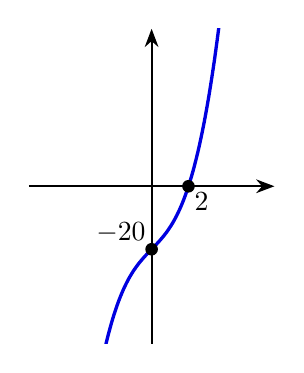
\begin{tikzpicture}
			\begin{scope}[xscale=.78]
				\draw[cstaxis] (-2,0)--(2,0);
				\draw[cstaxis] (0,-2)--(0,2);
				\clip (-2,-2) rectangle (2,2);
				\begin{scope}[xscale=.3,yscale=.04]
					\draw[cstcurve,main,domain=-3:4,smooth] plot (\x,{\x*\x*\x+6*\x-20});
					\coordinate (A) at (2,0);
					\coordinate (B) at (0,-20);
				\end{scope}
				\draw[inner sep=2pt]
					(A) node[below right] {$2$}
					(B) node[above left] {$-20$};
			\end{scope}
			\begin{scope}[cstdot]
				\fill (A) circle;
				\fill (B) circle;
			\end{scope}
		\end{tikzpicture}}
	\end{solution}
\end{frame}


\begin{frame}{三次方程的根\noexer}
	\beqskip{1pt}
	\onslide<+->
	\begin{example}[nearnext]
		解方程 $x^3-7x+6=0$.
	\end{example}
	\onslide<+->
	\begin{solution}[nearprev,sidepic,righthand width=2.7cm,leftupper=0mm]
		\begin{itemize}
			\item 类似地 $x=u+v$, 其中 $u^3+v^3=-6$, $uv=\frac73$.
			\item 于是 $u^3,v^3$ 满足一元二次方程 $X^2+6X+\frac{343}{27}=0$.
			\item 这个方程没有实数解, 我们可以强行解得 
		\end{itemize}
		\onslide<+->{%
		\[
			u^3=-3+\dfrac{10}9\sqrt{-3},\ 
			\visible<+->{u=\frac{3+2\sqrt{-3}}3,\frac{-9+\sqrt{-3}}6,\frac{3-5\sqrt{-3}}6,}
		\]}
		\begin{itemize}
			\item $v=\dfrac{3-2\sqrt{-3}}3,\dfrac{-9-\sqrt{-3}}6,\dfrac{3+5\sqrt{-3}}6$,
			\item $x=u+v=2,-3,1$.
		\end{itemize}
		\tcblower
		\onslide<+->{%
		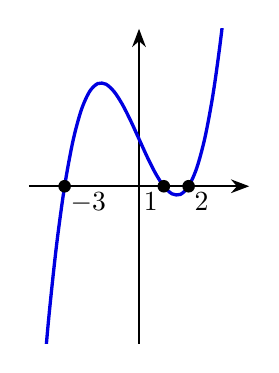
\begin{tikzpicture}
			\begin{scope}[xscale=.7]
				\def\a{-3}
				\def\b{1}
				\def\c{2}
				\draw[cstaxis] (-2,0)--(2,0);
				\draw[cstaxis] (0,-2)--(0,2);
				\clip (-2,-2) rectangle (2,2);
				\begin{scope}[xscale=.45,yscale=.1]
					\draw[cstcurve,main,domain=-4:4,smooth] plot (\x,{(\x-\a)*(\x-\b)*(\x-\c)});
					\coordinate (A) at (\a,0);
					\coordinate (B) at (\b,0);
					\coordinate (C) at (\c,0);
				\end{scope}
				\draw[inner sep=2pt]
					(A) node[below right] {$-3$}
					(B) node[below left] {$1$}
					(C) node[below right] {$2$};
			\end{scope}
			\begin{scope}[cstdot]
				\fill (A) circle;
				\fill (B) circle;
				\fill (C) circle;
			\end{scope}
		\end{tikzpicture}}
	\end{solution}
	\endgroup
\end{frame}


\begin{frame}{三次方程的根\noexer}
	\begin{itemize}
		\item 一般地, 方程 $x^3+px+q=0$ 的解为($p=0$ 情形较简单, 这里不考虑)
		\[
			x=u-\frac p{3u},\quad u^3=-\frac q2+\sqrt{\Delta},\quad \Delta=\frac{q^2}4+\frac{p^3}{27}.
		\]
		\item 通过分析函数图像的极值点可以知道:
	\end{itemize}
	\begin{center}
		\begin{tikzpicture}[visible on=<3->]
			\begin{scope}[scale=.65,
				declare function={
					f(\x)=\x*\x*\x-3*\x;
				}
			]
				\def\a{2.5}
				\draw[cstaxis] (-2,0)--(2,0);
				\draw[cstaxis] (0,-2) node[below] {$\Delta>0$, 有 $1$ 个根}--(0,2);
				\clip (-2,-2) rectangle (2,2);
				\begin{scope}[xscale=.35,yscale=.1]
					\draw[cstcurve,main,domain=-3:4,smooth] plot (\x,{f(\x)-f(\a)});
					\coordinate (A) at (\a,0);
				\end{scope}
			\end{scope}
			\fill[cstdot] (A) circle;
			\begin{scope}[visible on=<4->,xshift=5cm]
				\begin{scope}[scale=.65]
					\def\a{-2}
					\def\b{1}
					\draw[cstaxis] (-2,0)--(2,0);
					\draw[cstaxis] (0,-2) node[below,align=center] {$\Delta=0$, 有 $2$ 个根\\$x=-\sqrt[3]{4q},\half\sqrt[3]{4q}$ ($2$重).}--(0,2);
					\clip (-2,-2) rectangle (2,2);
					\begin{scope}[xscale=.35,yscale=.1]
						\draw[cstcurve,main,domain=-4:3,smooth] plot ({\x},{(\x-\a)*(\x-\b)*(\x-\b)});
						\coordinate (A) at (\a,0);
						\coordinate (B) at (\b,0);
					\end{scope}
				\end{scope}
				\begin{scope}[cstdot]
					\fill (A) circle;
					\fill (B) circle;
				\end{scope}
			\end{scope}
			\begin{scope}[visible on=<5->,xshift=10cm]
				\begin{scope}[scale=.65]
					\def\a{-3}
					\def\b{.5}
					\def\c{2.5}
					\draw[cstaxis] (-2,0)--(2,0);
					\draw[cstaxis] (0,-2) node[below] {$\Delta<0$, 有 $3$ 个根}--(0,2);
					\clip (-2,-2) rectangle (2,2);
					\begin{scope}[xscale=.3,yscale=.05]
						\draw[cstcurve,main,domain=-5:5,smooth] plot ({\x},{(\x-\a)*(\x-\b)*(\x-\c)});
						\coordinate (A) at (\a,0);
						\coordinate (B) at (\b,0);
						\coordinate (C) at (\c,0);
					\end{scope}
				\end{scope}
				\begin{scope}[cstdot]
					\fill (A) circle;
					\fill (B) circle;
					\fill (C) circle;
				\end{scope}
			\end{scope}
		\end{tikzpicture}
	\end{center}
\end{frame}


\begin{frame}{三次方程的根\noexer}
	\begin{itemize}
		\item 由此可见, 若想使用求根公式, 就\alert{必须接受负数开方}.
		\item 那么为什么当 $\Delta<0$ 时, 从求根公式一定能得到 $3$ 个实根呢?
		\item 这个问题在我们学习了第一章的内容之后可以得到回答.
		\item 尽管在十六世纪, 人们已经得到了三次方程的求根公式, 然而对其中出现的虚数, 却是难以接受.
		\item 莱布尼兹曾说: {\color{third}\itshape 圣灵在分析的奇观中找到了超凡的显示, 这就是那个理想世界的端兆, 那个介于存在与不存在之间的两栖物, 那个我们称之为虚的 $-1$ 的平方根。}
		\item 不过, 现在我们可以用更为现代和严格的语言来引入复数.
	\end{itemize}
\end{frame}

\subsection{复数的概念}

\begin{frame}{复数的定义}
	\begin{itemize}
		\item 现在我们来正式介绍复数的概念.
		\item 为了避免记号 $\sqrt{-1}$ 带来的歧义, 我们先引入抽象符号 $\ii$, 再通过定义它的运算来构造复数.
	\end{itemize}
	\onslide<+->
	\begin{definition}
		固定一个记号 $\ii$, \emph{复数}就是形如 $z=x+y\ii$ 的元素, 其中 $x,y$ 均是实数, 且不同的 $(x,y)$ 对应不同的复数.
	\end{definition}
	\begin{itemize}
		\item 实数 $x$ 可以自然地看成复数 $x+0\ii$.
	\end{itemize}
\end{frame}


\begin{frame}{复平面}
	\begin{itemize}
		\item 回忆全体实数、有理数、整数、自然数构成的集合分别记作 $\BR,\BQ,\BZ,\BN$.
		\item 将\emph{全体复数记作 $\BC$}.
		\item 那么 $\BC$ 自然构成一个二维实线性空间, 且 $\{1,\ii\}$ 是一组基. 
		\item 因此它和平面上的点可以建立一一对应, 并将建立起这种对应的平面称为\emph{复平面}.
	\end{itemize}
	\onslide<+->
	\begin{center}
		\begin{tikzpicture}
			\begin{scope}
				\draw[cstaxis] (-.5,0)--(3,0);
				\draw[cstaxis] (0,-.5)--(0,2.5);
				\coordinate [label=below left:$0$] (O) at (0,0);
				\coordinate [label=above:\textcolor{second}{$z=x+y\ii$}] (A) at (2,1.5);
				\coordinate (B) at (2,0);
				\coordinate (C) at (0,1.5);
				\draw[cstdash] (B)--(A)--(C);
				\fill[cstdot,second] (A) circle;
				\draw[third,Latex-Latex,line width=.5mm] (2.8,1)--(4,1) node[midway,below,third] {一一对应};
			\end{scope}
			\begin{scope}[xshift=5cm]
				\coordinate [label=below left:$O$] (O) at (0,0);
				\coordinate [label=above:\textcolor{second}{$Z(x,y)$}] (A) at (2,1.5);
				\coordinate (B) at (2,0);
				\coordinate (C) at (0,1.5);
				\draw[cstdash] (B)--(A)--(C);
				\fill[cstdot,second] (A) circle;
				\draw[decorate,decoration={brace,amplitude=5},main,cstfill1] (O)--(B) node[midway,above=2mm] {$x$};
				\draw[decorate,decoration={brace,amplitude=5},main,cstfill1] (C)--(O) node[midway,right=2mm] {$y$};
				\draw[third,Latex-Latex,line width=.5mm] (2.8,1)--(4,1) node[midway,below,third] {一一对应};
				\draw[cstaxis] (-.5,0)--(3,0);
				\draw[cstaxis] (0,-.5)--(0,2.5);
			\end{scope}
			\begin{scope}[xshift=10cm]
				\draw[cstaxis] (-.5,0)--(3,0);
				\draw[cstaxis] (0,-.5)--(0,2.5);
				\coordinate [label=below left:$O$] (O) at (0,0);
				\coordinate [label=above:\textcolor{second}{$\overrightarrow{OZ}=(x,y)$}] (A) at (2,1.5);
				\draw[cstcurve,cstra,second] (O)--(A);
			\end{scope}
		\end{tikzpicture}
	\end{center}
\end{frame}


\begin{frame}{实部和虚部, 虚数和纯虚数}
	\onslide<+->
	\begin{itemize}
		\item $x,y$ 轴分别对应复平面的\emph{实轴}和\alert{虚轴}.
		\item 称 $z=x+y\ii$ 中 $x=\Re z$ 为 $z$ 的\emph{实部}; $y=\Im z$ 为 $z$ 的\alert{虚部}.
		\item 当虚部 $\Im z=0$ 时, $z$ 为实数, 它落在实轴上.
		\item 不是实数的复数是\textcolor{third}{\bf 虚数}.
		\item 当实部 $\Re z=0$ 且 \alert{$z\neq0$} 时, $z$ 为\alert{纯虚数}, 它落在虚轴上.
	\end{itemize}
	\onslide<1->
	\begin{figure}[hbpt]
		\centering
		\begin{minipage}{.48\textwidth}
			\raggedleft
			\begin{tikzpicture}
				\coordinate [label=below left:$0$] (O) at (0,0);
				\coordinate (B) at (2,0);
				\coordinate (C) at (0,1.5);
				\draw[cstaxis] (-.5,0)--(3,0);
				\draw[cstaxis] (0,-.5)--(0,2.5);
				\begin{scope}[visible on=<3->]
					\draw[decorate,decoration={brace,amplitude=5},main,cstfill1] (B)--(O) node[midway,below=1.5mm] {$\Re z$};
					\draw[decorate,decoration={brace,amplitude=5},second,cstfill2] (C)--(O) node[midway,right=1.5mm] {$\Im z$};
					\coordinate [label=above:\textcolor{third}{$z=x+y\ii$}] (A) at (2,1.5);
					\draw[cstdash] (B)--(A)--(C);
					\fill[cstdot,third] (A) circle;
				\end{scope}
				\begin{scope}[visible on=<2->]
					\coordinate [label=above:\textcolor{main}{实轴}] (R) at (3,0);
					\coordinate [label=right:\textcolor{second}{虚轴}] (I) at (0,2.5);
					\draw[cstaxis,main] (-.5,0)--(R);
					\draw[cstaxis,second] (0,-.5)--(I);
				\end{scope}
				\draw[main,->,thick,visible on=<4->] (-2,.2)-|(.6,0);
				\draw[second,->,thick,visible on=<6->] (-2,1.3)--(0,1.3);
				\draw 
					(-2,.1) node[cstnode,draw=main,text=main,visible on=<4->] {实数}
					(-2,1.2) node[align=center,cstnode,draw=second,text=second,visible on=<6->] {纯虚数\\不含原点};
			\end{tikzpicture}
		\end{minipage}
		\begin{minipage}{.48\textwidth}
			\centering
			\begin{tikzpicture}
				\filldraw[cstcurve,cstfill] (.8,0) circle (2.6 and 2);
				\coordinate (R) at (0,-.8);
				\filldraw[cstcurve,main,fill=white,visible on=<4->] (R) circle (1.2 and .7);
				\coordinate (I) at (0,.8);
				\draw (R) node[align=center,main,visible on=<4->] {实数 \\$0,1,\sqrt2,\pi,\ee$};
				\draw (I) node[align=center,second,visible on=<6->] {纯虚数 \\$\ii,-\ii ,\pi\ii$};
				\draw[cstcurve,second,visible on=<6->] (I) circle (1.2 and .7);
				\draw 
					(3.7,0) node[align=center] {全\\体\\复\\数}
					(2,0) node[align=center,third,visible on=<5->] {虚数 \\$\ii,\pi\ii,\frac{-1+\sqrt 3 \ii}2$};
			\end{tikzpicture}
		\end{minipage}
	\end{figure}
\end{frame}


\begin{frame}{例题:判断实数和纯虚数}
	\onslide<+->
	\begin{example}[nearnext]
		实数 $x$ 取何值时, $z=(x^2+3x-4)+(x^2+5x-6)\ii$ 是:
		\begin{subexample}[2]
			\item 实数;
			\item 纯虚数.
		\end{subexample}
	\end{example}
	\onslide<+->
	\begin{solution}[nearprev]
		\begin{enumerate}
			\item $\Im z=x^2+5x-6=0$, 即 $x=1$ 或 $-6$.
			\item $\Re z=x^2+3x-4=0$, 即 $x=1$ 或 $-4$.
				\onslide<+->{%
					但同时要求 $\Im z=x^2+5x-6\neq 0$, 因此 $x\neq 1$.
				}\onslide<+->{%
					故 $x=-4$.
				}
		\end{enumerate}
	\end{solution}
	\onslide<+->
	\begin{exercise}
		若 $x^2(1+\ii)-x(5+4\ii)+4+3\ii$ 是纯虚数, 则实数 $x=$\fillblankframe{$4$}.
	\end{exercise}
\end{frame}


\subsection{复数的代数运算}


\begin{frame}{复数的加法与减法}
	\begin{itemize}
		\item 设 $z_1=x_1+y_1\ii,z_2=x_2+y_2\ii$.
		\item 定义复数的\emph{加法}和\emph{减法}:
		\[
			z_1+z_2=(x_1+x_2)+(y_1+y_2)\ii,\quad
			z_1-z_2=(x_1-x_2)+(y_1-y_2)\ii.
		\]
		\item 复数的加减法与其对应的向量 $\overrightarrow{OZ}$ 的加减法是一致的.
	\end{itemize}
	\onslide<1->
	\begin{center}
		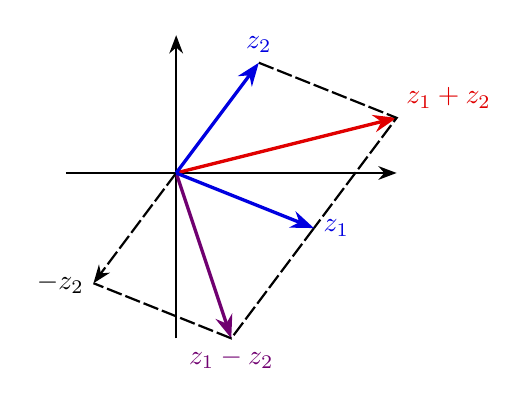
\begin{tikzpicture}[scale=.7]
			\draw[cstaxis] (-2,0)--(4,0);
			\draw[cstaxis] (0,-3)--(0,2.5);
			\coordinate (O) at (0,0);
			\coordinate [label=right:\textcolor{main}{$z_1$}] (Z1) at (2.5,-1);
			\coordinate [label=above:\textcolor{main}{$z_2$}] (Z2) at (1.5,2);
			\begin{scope}[visible on=<3->]
				\coordinate [label=above right:\textcolor{second}{$z_1+z_2$}] (P) at ($(Z1)+(Z2)$);
				\draw[cstcurve,cstra,second] (O)--(P);
				\draw[cstdash] (Z2)--(P)--(Z1);
			\end{scope}
			\begin{scope}[visible on=<4->]
				\coordinate [label=below:\textcolor{third}{$z_1-z_2$}] (M) at ($(Z1)-(Z2)$);
				\coordinate [label=left:{$-z_2$}] (neg) at ($(O)-(Z2)$);
				\draw[cstcurve,cstra,third] (O)--(M);
				\draw[cstdash,cstra] (O)--(neg);
				\draw[cstdash] (Z1)--(M)--(neg);
			\end{scope}
			\draw[cstcurve,cstra,main] (O)--(Z1);
			\draw[cstcurve,cstra,main] (O)--(Z2);
		\end{tikzpicture}
	\end{center}
\end{frame}


\begin{frame}{复数的乘除法}
	\begin{itemize}
		\item \alert{规定 $\ii\cdot \ii=-1$}.
		\item 定义复数的\emph{乘法}:
		\begin{align*}
			z_1\cdot z_2&
			=(x_1+y_1\ii)(x_2+y_2\ii)
			=x_1\cdot x_2+x_1\cdot y_2\ii+y_1\ii\cdot x_2+y_1\ii\cdot y_2\ii\\
			&=(x_1x_2-y_1y_2)+(x_1y_2+x_2y_1)\ii.
		\end{align*}
		\item 此时加法/乘法交换律, 结合律以及乘法分配律均成立.
		\item 待定系数可得复数的\emph{除法}定义为:
		\[
			\frac{z_1}{z_2}
			=\frac{(x_1+y_1\ii)(x_2-y_2\ii)}{x_2^2+y_2^2}
			=\frac{x_1x_2+y_1y_2}{x_2^2+y_2^2}+\frac{x_2y_1-x_1y_2}{x_2^2+y_2^2}\ii.
		\]
		\item 对于正整数 $n$, 定义 $z$ 的 \emph{$n$ 次幂}为 $n$ 个 $z$ 相乘.
		\item 当 $z\neq 0$ 时, 还可以定义 $z^0=1,z^{-n}=\dfrac1{z^n}$.
	\end{itemize}
\end{frame}


\begin{frame}{例: 单位根}
	\onslide<+->
	\begin{example}
		\begin{enumerate}
			\item $\ii^2=-1,\ii^3=-\ii ,\ii^4=1$.
			\onslide<+->{%
			一般地, 对于整数 $n$, 
			\[
				\ii^{4n}=1,\quad \ii^{4n+1}=i,\quad
				\ii^{4n+2}=-1,\quad \ii^{4n+3}=-\ii.
			\]
			}
			\vspace{-\baselineskip}
			\item 令 $\omega=\dfrac{-1+\sqrt 3\ii}2$, 则 $\omega^2=\dfrac{-1-\sqrt3\ii}2,\omega^3=1$.
			\item 令 $z=1+\ii$, \onslide<+->{则
			\[
				z^2=2\ii,\quad z^3=-2+2\ii,\quad z^4=-4,\quad z^8=16=2^4.
			\]}
		\end{enumerate}
		\bigdel\bigdel
	\end{example}
	\begin{itemize}
		\item 将满足 $z^n=1$ 的复数 $z$ 称为 \emph{$n$ 次单位根}.
		\item 那么 $1,\ii,-1,-\ii $ 是 $4$ 次单位根, $1,\omega,\omega^2$ 是 $3$ 次单位根, $-\omega$ 是 $6$ 次单位根.
	\end{itemize}
\end{frame}


\begin{frame}{例: 代数式的计算}
	\begin{itemize}
		\item 实数情形的等差数列求和公式、等比数列求和公式、二项式展开、平方差公式等在复数情形也成立.
	\end{itemize}
	\onslide<+->
	\begin{example}[nearnext]
		化简 $1+\ii+\ii^2+\dots+\ii^{1000}$.
	\end{example}
	\onslide<+->
	\begin{solution}[nearprev]
		根据等比数列求和公式, $1+\ii+\ii^2+\dots+\ii^{1000}
			=\dfrac{\ii^{1001}-1}{\ii-1}
			\visible<+->{=\dfrac{\ii-1}{\ii-1}=1.}$
	\end{solution}
	\onslide<+->
	\begin{exercise}
		化简 $\Bigl(\dfrac{1+\ii}{1-\ii}\Bigr)^{2026}$=\fillblankframe{$-1$}.
	\end{exercise}
\end{frame}


\subsection{共轭复数}


\begin{frame}{共轭复数的定义}
	\onslide<+->
	\begin{definition}
		称 $z$ 在复平面关于实轴的对称点为它的\emph{共轭复数 $\ov z$}.
		换言之, $\ov{x+y\ii}=x-y\ii$.
	\end{definition}
	\onslide<+->
	\begin{exercise}
		$z$ 关于虚轴的对称点是\fillblankframe{$-\ov z$}.
	\end{exercise}
\end{frame}

\begin{frame}{共轭复数的性质}
	\begin{itemize}
		\item 从定义出发, 不难验证共轭复数满足如下性质:
		\begin{enumerate}\bf
			\item $z$ 是 $\ov z$ 的共轭复数.\hfill\alert{共轭是一种对合}
			\item $\ov{z_1\pm z_2}=\ov{z_1}\pm\ov{z_2},\ 
			\ov{z_1\cdot z_2}=\ov{z_1}\cdot\ov{z_2},\ 
			\ov{\Bigl(\dfrac{z_1}{z_2}\Bigr)}=\dfrac{~\ov{z_1}~}{~\ov{z_2}~}$.
			\hfill \alert{共轭复数和四则运算交换}
			\item $z\ov{z}=(\Re z)^2+(\Im z)^2$.
			\item $z+\ov z=2\Re z,\ z-\ov z=2\ii\Im z$.
			\hfill \alert{$x,y$ 和 $z,\ov z$ 可相互表示}
			\item $z=\ov z\iff z$ 是实数; $z=-\ov z\iff z$ 是纯虚数或 $z=0$.\hfill\alert{判断实数和纯虚数}
		\end{enumerate}
		\item 这些性质意味着使用共轭复数进行计算和证明,往往比直接使用 $x,y$ 表达的形式更简单.
	\end{itemize}
\end{frame}


\begin{frame}{例题:共轭复数证明等式}
	\onslide<+->
	\begin{example}
		证明 $z_1\cdot\ov{z_2}-\ov{z_1}\cdot z_2=2\ii\Im(z_1\cdot\ov{z_2})$.
	\end{example}
	\onslide<+->
	我们可以设 $z_1=x_1+y_1\ii,z_2=x_2+y_2\ii$, 然后代入等式两边化简并比较实部和虚部得到.
	\onslide<+->
	但我们利用共轭复数可以更简单地证明它.
	\onslide<+->
	\begin{proof}[leftupper=0mm]
		\begin{itemize}
			\item 由于 $\ov{z_1\cdot\ov{z_2}}=\ov{z_1}\cdot\ov{\ov{z_2}}=\ov{z_1}\cdot z_2$, 
			\item 因此
			\[
				z_1\cdot\ov{z_2}-\ov{z_1}\cdot z_2
				=z_1\cdot\ov{z_2}-\ov{z_1\cdot\ov{z_2}}
				=2\ii\Im(z_1\cdot\ov{z_2}).\qedhere
			\]
		\end{itemize}
	\end{proof}
\end{frame}


\begin{frame}{例题:共轭复数判断实数}
	\onslide<+->
	\begin{example}[nearnext]
		设 $z=x+y\ii$ 是虚数.
		证明: $x^2+y^2=1$ 当且仅当 $z+\dfrac 1z$ 是实数.
	\end{example}
	\onslide<+->
	\begin{proof}[nearprev,leftupper=0mm]
		\begin{itemize}
			\item $z+\dfrac 1z$ 是实数等价于
				$z+\dfrac 1z=\ov{\Bigl(z+\dfrac 1z\Bigr)}=\ov z+\dfrac1{~\ov z~}$,
			\item 等价于
			\[
				z-\ov z=\frac1{~\ov z~}-\frac1z=\frac{z-\ov z}{z\ov z},\quad (z-\ov z)(z\ov z-1)=0.
			\]
			\item 由 $z$ 是虚数可知 $z\neq \ov z$.
			\item 故上述等式等价于 $z\ov z=1$, 即 $x^2+y^2=1$.\qedhere
		\end{itemize}
	\end{proof}
\end{frame}


\begin{frame}{例: 复数的代数计算}
	\onslide<+->
	由于 $z\ov z$ 是一个实数,
	\onslide<+->
	因此在做复数的除法运算时, 可以利用下式将其转化为乘法:
	\[
		\dfrac{z_1}{z_2}=\dfrac{z_1\ov{z_2}}{z_2\ov{z_2}}=\dfrac{z_1\ov{z_2}}{x_2^2+y_2^2}.
	\]
	\bigdel
	\onslide<+->
	\begin{example}[nearnext]
		$z=-\dfrac1\ii-\dfrac{3\ii}{1-\ii }$, 求 $\Re z,\Im z$ 以及 $z\ov z$.
	\end{example}
	\onslide<+->
	\begin{solution}[nearprev]
		\[
			z=-\frac1\ii-\frac{3\ii}{1-\ii }
			\onslide<+->{=\ii-\frac{3\ii-3}2=\frac32-\half \ii,}
		\]
		\onslide<+->{%
		\[
			\Re z=\frac32,\quad\Im z=-\half ,\quad
			z\ov z=\Bigl(\frac32\Bigr)^2+\Bigl(-\half\Bigr)^2=\frac52.
		\]
		}
		\bigdel
	\end{solution}
\end{frame}


\begin{frame}{例: 复数的代数计算}
	\onslide<+->
	\begin{example}[nearnext]
		设 $z_1=5-5\ii,z_2=-3+4\ii$, 求 $\ov{\Bigl(\dfrac{z_1}{z_2}\Bigr)}$.
	\end{example}
	\onslide<+->
	\begin{solution}[nearprev]
		\begin{align*}
			\frac{z_1}{z_2}&=\frac{5-5\ii}{-3+4\ii}
			\onslide<+->{=\frac{(5-5\ii)(-3-4\ii)}{(-3)^2+4^2}}\\
			&\onslide<+->{=\frac{(-15-20)+(-20+15)\ii}{25}}
			\onslide<+->{=-\frac75-\frac15\ii,}
		\end{align*}
		\onslide<+->{%
			因此 $\ov{\Bigl(\dfrac{z_1}{z_2}\Bigr)}=-\dfrac75+\dfrac15\ii$.
		}
	\end{solution}
\end{frame}



% \begin{frame}{复数域\noexer}
% 	\begin{itemize}
% 		\item 复数全体构成一个\emph{域}.
% 		\item 所谓的域, 是指带有如下内容和性质的集合
% 		\begin{itemize}\bf
% 			\item 包含 $0,1$, 且有四则运算;
% 			\item 满足加法结合/交换律, 乘法结合/交换/分配律;
% 			\item 对任意 $a$, $a+0=a\times 1=a$.
% 		\end{itemize}
% 		\item 有理数全体 $\BQ$, 实数全体 $\BR$ 也构成域, 它们是 $\BC$ 的子域.
% 		\item 与有理数域和实数域有着本质不同的是, 复数域是\emph{代数闭域}:
% 		\item 对于任何次数 $n\ge 1$ 的复系数多项式
% 		\[
% 			p(z)=z^n+c_{n-1}z^{n-1}+\cdots+c_1z+c_0,
% 		\]
% 		都存在复数 $z_0$ 使得 $p(z_0)=0$.
% 		\item 由此不难知道, 复系数多项式可以因式分解成一次多项式的乘积.
% 		\item 我们会在第五章证明该结论.
% 	\end{itemize}
% \end{frame}


% \begin{frame}{复数域不是有序域\noexer}
% 	\begin{itemize}
% 		\item \onslide<+->
% 	\end{itemize}
% 	在 $\BQ,\BR$ 上可以定义出一个好的大小关系,
% 	\onslide<+->
% 	换言之它们是有序域, 即存在一个满足下述性质的 $>$:
% 	\begin{itemize}\bf
% 		\item 若 $a\neq b$, 则要么 $a>b$, 要么 $b>a$;
% 		\item 若 $a>b$, 则对于任意 $c$, $a+c>b+c$;
% 		\item 若 $a>b,c>0$, 则 $ac>bc$.
% 	\end{itemize}
% 	\onslide<+->
% 	而 \alert{$\BC$ 却不是有序域}.
% 	\onslide<+->
% 	若 $\ii>0$, 则
% 	\[
% 		-1=\ii\cdot \ii>0,\quad -\ii =-1\cdot \ii>0.
% 	\]
% 	\onslide<+->
% 	于是 $0>\ii$, 矛盾! 同理 $\ii<0$ 也不可能.
% \end{frame}

\section{复数的三角与指数形式}

\subsection{复数的模和辐角}
\begin{frame}{复数的极坐标形式}
	\onslide<+->
	由平面的极坐标表示, 我们可以得到复数的另一种表示方式.
	\onslide<+->
	以 $0$ 为极点, 正实轴为极轴, 逆时针为极角方向可以自然定义出复平面上的极坐标系.
	\onslide<+->
	\begin{center}
		\begin{minipage}{.4\textwidth}
			\centering
			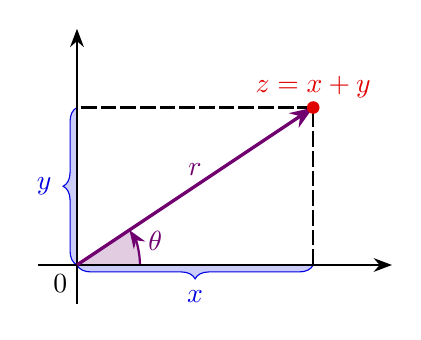
\begin{tikzpicture}
				\coordinate [label=below left:$0$] (O) at (0,0);
				\coordinate [label=above:\textcolor{second}{$z=x+y\ii$}] (Z) at (3,2);
				\coordinate (X) at (3,0);
				\coordinate (Y) at (0,2);
				\draw[decorate,decoration={brace,amplitude=5},main,cstfill1] (X)--(O) node[midway,below=2mm] {$x$};
				\draw[decorate,decoration={brace,amplitude=5},main,cstfill1] (O)--(Y) node[midway,left=2mm] {$y$};
				\draw[third,thick,cstra] pic [cstfill3,draw=third, "$\theta$", angle eccentricity=1.3, angle radius=0.8cm] {angle=X--O--Z};
				\draw[cstaxis] (-.5,0)--(4,0);
				\draw[cstaxis] (0,-.5)--(0,3);
				\draw[cstcurve,third,cstra] (O)--(Z) node[midway,above,third] {$r$};
				\draw[cstdash] (X)--(Z)--(Y);
				\fill[cstdot,second] (Z) circle;
			\end{tikzpicture}
		\end{minipage}
		\begin{minipage}{.56\textwidth}
			\centering
			\onslide<4->{
			\[ x=r\cos\theta,\qquad y=r\sin\theta,
	\]
			\[r=\sqrt{x^2+y^2},\qquad \theta=\arctan\dfrac yx\text{ 或 }\arctan\dfrac yx\pm\pi.\]}
		\end{minipage}
	\end{center}
	\vspace{-\baselineskip}

	\onslide<+->
	\onslide<+->
	\begin{definition}
		\begin{itemize}
			\item 称 $r$ 为 $z$ 的\emph{模}, 记为 \emph{$|z|=r$}.
			\item 称 $\theta$ 为 $z$ 的\emph{辐角}, 记为 \emph{$\Arg z=\theta$}.
			\onslide<+->{约定 \alert{$0$ 的辐角没有定义}.}
		\end{itemize}
	\end{definition}
\end{frame}


\begin{frame}{辐角主值}
	\onslide<+->
	任意 $z\neq 0$ 的辐角有无穷多个.
	\onslide<+->
	我们固定选择其中位于 $(-\pi,\pi]$ 的那个, 并称之为\emph{辐角主值}或\emph{辐角主值}, 记作 $\emphm{\arg z}$.
	\onslide<+->
	那么 $\emphm{\Arg z=\arg z+2k\pi, k\in\BZ}$.

	\onslide<2->
	\begin{figure}[hbpt]
		\centering
		\begin{minipage}{.46\textwidth}
			\onslide<4->{
			\[\arg z=\begin{cases}
				\visible<4->{\emphn{\arctan\dfrac yx,}}&\visible<4->{\emphn{x>0;}}\vspace{1ex}\\
				\visible<5->{\alertn{\arctan\dfrac yx+\pi,}}&\visible<5->{\alertn{x<0,y\ge0;}}\vspace{1ex}\\
				\visible<6->{\color{third}{\arctan\dfrac yx-\pi,}}&\visible<6->{\color{third}{x<0,y<0;}}\\
				\visible<7->{\color{fourth}{\dfrac\pi2,}}&
				\visible<7->{\color{fourth}{x=0,y>0;}}\\
				\visible<7->{\color{fourth}{-\dfrac\pi2,}}&
				\visible<7->{\color{fourth}{x=0,y<0.}}
				\end{cases}\]}
		\end{minipage}
		\begin{minipage}{.52\textwidth}
			\begin{tikzpicture}
				\draw[cstaxis](-2.5,0)->(2.5,0); 
				\draw[cstaxis](0,-2)->(0,2);
				\draw[cstaxis,main,cstwla] (-1.5,0) arc(180:-180:1.5);
				\filldraw[cstdote,draw=main] (-1.5,-.07) circle;
				\begin{scope}[visible on=<4->]
					\coordinate [label=above:\textcolor{main}{$0$}] (A) at (1.7,0);
					\fill[cstdot,main] (A) circle;
					\coordinate [label=above right:\textcolor{main}{$\arctan\dfrac yx$}] (B) at (.9,.9);
					\fill[cstdot,main] (B) circle;
					\coordinate [label=right:\textcolor{main}{$\arctan\dfrac yx$}] (C) at (1.4,-.9);
					\fill[cstdot,main] (C) circle;
				\end{scope}
				\begin{scope}[visible on=<5->]
					\coordinate [label=above left:\textcolor{second}{$\arctan\dfrac yx+\pi$}] (D) at (-1.1,.8);
					\fill[cstdot,second] (D) circle;
					\coordinate [label=below:\textcolor{second}{$\pi$}] (E) at (-.9,0);
					\fill[cstdot,second] (E) circle;
				\end{scope}
				\begin{scope}[visible on=<6->]
					\coordinate [label=left:\textcolor{third}{$\arctan\dfrac yx-\pi$}] (F) at (-1.6,-.7);
					\fill[cstdot,third] (F) circle;
				\end{scope}
				\begin{scope}[visible on=<7->]
					\coordinate [label=left:\textcolor{fourth}{$\dfrac\pi2$}] (G) at (0,.5);
					\fill[cstdot,fourth] (G) circle;
					\coordinate [label=right:\textcolor{fourth}{$-\dfrac\pi2$}] (H) at (0,-.6);
					\fill[cstdot,fourth] (H) circle;
				\end{scope}
			\end{tikzpicture}
		\end{minipage}
	\end{figure}
	\vspace{-\baselineskip}
	\onslide<9->
	注意 \alert{$\arg \ov z=-\arg z$ 未必成立}, 仅当 $z$ 不是负实数和 $0$ 时成立.
\end{frame}


\begin{frame}{复数模的性质}\small
	\onslide<+->
	复数的模满足如下性质:
	\begin{figure}[hbpt]
		\centering
		\begin{minipage}{.48\textwidth}
			\begin{itemize}\bf
				\item $z\ov z=|z|^2=|\ov z|^2$;
				\item $\abs{\Re z},\abs{\Im z}\le |z|\le\abs{\Re z}+\abs{\Im z}$;
			\end{itemize}
		\end{minipage}
		\begin{minipage}{.48\textwidth}
			\begin{itemize}\bf
				\item $\big||z_1|-|z_2|\big|\le|z_1\pm z_2|\le|z_1|+|z_2|$;
				\item $|z_1+z_2+\cdots+z_n|\le|z_1|+|z_2|+\cdots+|z_n|$.
			\end{itemize}
		\end{minipage}
	\end{figure}
	\begin{center}
		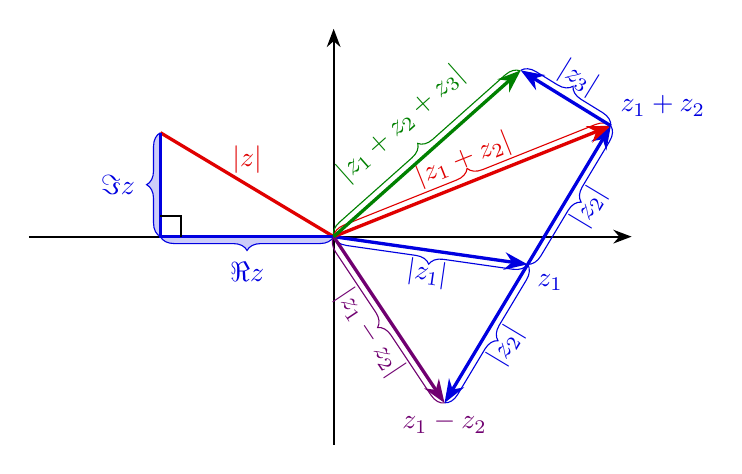
\begin{tikzpicture}[visible on=<3->,scale=.88]
			\draw[cstaxis] (-4.4,0)--(4.3,0);
			\draw[cstaxis] (0,-3)--(0,3);
			\coordinate (O) at (0,0);
			\coordinate (Z) at (-2.5,1.5);
			\coordinate (R) at (-2.5,0);
			\draw[decorate,decoration={brace,amplitude=5},main,cstfill1] (O)--(R) node[midway,below=2mm,main] {$\abs{\Re z}$};
			\draw[decorate,decoration={brace,amplitude=5},main,cstfill1] (R)--(Z) node[midway,left=2mm,main] {$\abs{\Im z}$};
			\draw[cstcurve,second] (O)--(Z) node[midway,above,second] {$|z|$};
			\draw[cstcurve,main] (Z)--(R)--(O);
			\draw[thick] (R) ++(0,.3)--++(.3,0)--++(0,-.3);
	
			\begin{scope}[visible on=<4->]
				\coordinate [label=below right:\textcolor{main}{$z_1$}] (Z1) at (2.8,-.4);
				\coordinate (Z2) at (1.2,2);
				\coordinate [label=above right:\textcolor{main}{$z_1+z_2$}] (P) at ($(Z1)+(Z2)$);
				\coordinate [label=below:\textcolor{third}{$z_1-z_2$}] (M) at ($(Z1)-(Z2)$);
				\draw[decorate,decoration={brace,amplitude=5},main] (Z1)--(O) node[midway,below,sloped] {$|z_1|$};
				\draw[decorate,decoration={brace,amplitude=5},main] (P)--(Z1) node[midway,below,sloped] {$|z_2|$};
				\draw[decorate,decoration={brace,amplitude=5},second] (O)--(P) node[midway,above,sloped] {$|z_1+z_2|$};
				\draw[decorate,decoration={brace,amplitude=5},main] (Z1)--(M) node[midway,below,sloped] {$|z_2|$};
				\draw[decorate,decoration={brace,amplitude=5},third] (M)--(O) node[midway,below,sloped] {$|z_1-z_2|$};
				\begin{scope}[cstcurve,cstra]
					\draw[main] (O)--(Z1);
					\draw[main] (Z1)--(P);
					\draw[second] (O)--(P);
					\draw[third] (O)--(M);
					\draw[main] (Z1)--(M);
				\end{scope}
			\end{scope}

			\begin{scope}[visible on=<5->]
				\coordinate (A) at (2.7,2.4);
				\draw[decorate,decoration={brace,amplitude=5},main] (A)--(P) node[midway,above,sloped] {$|z_3|$};
				\draw[decorate,decoration={brace,amplitude=5},fourth] (O)--(A) node[midway,above=2mm,sloped] {$|z_1+z_2+z_3|$};
				\begin{scope}[cstcurve,cstra]
					\draw[main] (P)--(A);
					\draw[fourth] (O)--(A);
				\end{scope}
			\end{scope}
		\end{tikzpicture}
	\end{center}
\end{frame}


\begin{frame}{例题:共轭复数解决模的等式}
	\beqskip{0pt}
	\onslide<+->
	\begin{example}
		证明
		\begin{enumerate}
			\item $|z_1z_2|=|z_1\ov{z_2}|=|z_1|\cdot|z_2|$;
			\item $|z_1+z_2|^2=|z_1|^2+|z_2|^2+2\Re(z_1\ov{z_2})$.
		\end{enumerate}
	\end{example}

	\onslide<+->
	\begin{proof}
		\begin{enumerate}
			\item 因为
				\[|z_1z_2|^2=z_1z_2\cdot\ov{z_1}\ov{z_2}
				=z_1z_2\ov{z_1}\ov{z_2}=|z_1|^2\cdot|z_2|^2,
	\]
				\onslide<+->{%
					所以 $|z_1z_2|=|z_1|\cdot|z_2|$.
				}\onslide<+->{%
					因此 $|z_1\ov{z_2}|=|z_1|\cdot|\ov{z_2}|=|z_1|\cdot|z_2|$.
				}
			\item 因为
				\begin{align*}
					\text{左边}&=(z_1+z_2)(\ov{z_1}+\ov{z_2})
					=z_1\ov{z_1}+z_2\ov{z_2}+z_1\ov{z_2}+\ov{z_1}z_2,\\
					\text{右边}&=z_1\ov{z_1}+z_2\ov{z_2}+z_1\ov{z_2}+\ov{z_1\ov{z_2}},
				\end{align*}
				\onslide<+->{%
					而 $\ov{z_1\ov{z_2}}=\ov{z_1}z_2$, 所以两侧相等.\qedhere
				}
		\end{enumerate}
	\end{proof}
	\endgroup
\end{frame}


\subsection{复数的三角形式和指数形式}
\begin{frame}{复数的三角形式和指数形式}
	\onslide<+->
	由 $x=r\cos\theta,y=r\sin\theta$ 可得
	\onslide<+->
	\begin{definition}[复数的三角形式]
	\[
		z=r(\cos\theta+\ii\sin\theta).\]	
	\end{definition}
	\onslide<+->
	定义 \alert{$\ee^{\ii\theta}=\exp(\ii\theta):=\cos\theta+\ii\sin\theta$} (欧拉恒等式),
	\onslide<+->
	则我们得到
	\begin{definition}[复数的指数形式]
	\[
		z=r\ee^{\ii\theta}=r\exp(\ii\theta).
	\]
	\end{definition}
	\onslide<+->
	这两种形式的等价的, 指数形式可以认为是三角形式的一种缩写方式.

	\onslide<+->
	求复数的三角和指数形式的\alert{关键在于计算模和辐角}.
\end{frame}


\begin{frame}{例: 求复数的三角和指数形式}
	\onslide<+->
	\begin{example}
		将 $z=-\sqrt{12}-2\ii$ 化成三角形式和指数形式.
	\end{example}

	\onslide<+->
	\begin{solution}
		$r=|z|=\sqrt{12+4}=4$.
		\onslide<+->{%
			由于 $z$ 在第三象限,
		}\onslide<+->{%
			因此
			\[\arg z=\arctan\frac{-2}{-\sqrt{12}}-\pi=\frac\pi6-\pi=-\frac{5\pi}6.
	\]
		}\onslide<+->{%
			故
			\[z=4\left[\cos\Bigl(-\frac{5\pi}6\Bigr)+\ii\sin\Bigl(-
			\frac{5\pi}6\Bigr)\right]=4\ee^{-\frac{5\pi\ii}6}.
	\]
		}
	\end{solution}
\end{frame}


\begin{frame}{例: 求复数的三角和指数形式}
	\beqskip{0pt}
	\onslide<+->
	\begin{example}
		将 $z=\sin\dfrac\pi5+\ii\cos\dfrac\pi5$ 化成三角形式和指数形式.
	\end{example}
	\onslide<+->
	\begin{solution}
		$r=|z|=1$.
		\onslide<+->{%
		由于 $z$ 在第一象限, 因此
		\[\arg z=\arctan\frac{\cos(\pi/5)}{\sin(\pi/5)}=\arctan\cot\frac\pi 5=\frac\pi2-\frac\pi5=\frac{3\pi}{10}.
		\]}\onslide<+->{%
		故
		\[
			z=\cos\frac{3\pi}{10}+\ii\sin\frac{3\pi}{10}=\ee^{\frac{3\pi\ii}{10}}.
		\]}
	\end{solution}
	\onslide<+->
	\begin{solution}[另解]
		\[
			z=\sin\frac\pi5+\ii\cos\frac\pi5
			\visible<+->{=\cos\Bigl(\frac\pi2-\frac\pi5\Bigr)+\ii\sin\Bigl(\frac\pi2-\frac\pi5\Bigr)}
			\visible<+->{=\cos\frac{3\pi}{10}+\ii\sin\frac{3\pi}{10}=\ee^{\frac{3\pi\ii}{10}}.}
		\]
	\end{solution}
	\endgroup
\end{frame}


\begin{frame}{例: 求复数的三角和指数形式}
	\onslide<+->
	求复数的三角或指数形式时, 我们只需要任取一个辐角就可以了, 不要求必须是辐角主值.

	\onslide<+->
	\begin{exercise}
		将 $z=\sqrt 3-3\ii$ 化成三角形式和指数形式.
	\end{exercise}

	\onslide<+->
	\begin{answer}
		$\displaystyle z=2\sqrt3\Bigl(\cos\frac{-\pi}3+\ii\sin\frac{-\pi}3\Bigr)
		=2\sqrt3\ee^{-\frac{\pi\ii}3}$, 写成 $\dfrac{5\pi}3$ 也可以.
	\end{answer}
\end{frame}


\begin{frame}{模为 $1$ 的复数}
	\onslide<+->
	两个模相等的复数之和的三角和指数形式形式较为简单.
	\onslide<+->
	\[
		\ee^{\ii\theta}+\ee^{\ii\varphi}
		=2\cos\frac{\theta-\varphi}2\ee^{\frac{\theta+\varphi}2\ii}.
	\]
	\vspace{-\baselineskip}
	\onslide<+->
	\begin{center}
		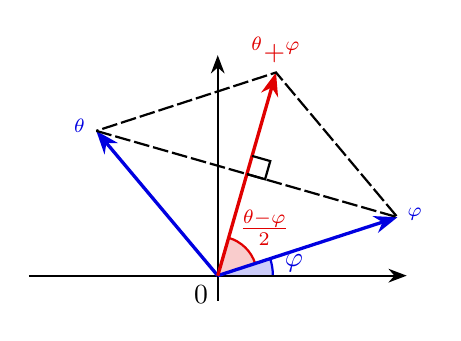
\begin{tikzpicture}[scale=.8]
			\coordinate [label=below left:0] (O) at (0,0);
			\coordinate [label=right:\textcolor{main}{$\ee^{\ii\varphi}$}] (Z1) at ({3*cos(18)},{3*sin(18)});
			\coordinate [label=left:\textcolor{main}{$\ee^{\ii\theta}$}] (Z2) at ({3*cos(130)},{3*sin(130)});
			\coordinate [label=above:\textcolor{second}{$\ee^{\ii\theta}+\ee^{\ii\varphi}$}] (P) at ($(Z1)+(Z2)$);
			\coordinate (M) at ($0.5*(P)$);
			\coordinate (X) at (2,0);
			\draw[thick,main] pic [cstfill1, draw=main,"$\varphi$", angle eccentricity=1.4, angle radius=0.7cm] {angle=X--O--Z1};
			\draw[thick,second] pic [cstfill2, draw=second, "$\frac{\theta-\varphi}2$", angle eccentricity=1.7] {angle=Z1--O--P};
			\draw[cstaxis] (-3,0)--(3,0);
			\draw[cstaxis] (0,-.4)--(0,3.5);
			\draw[cstcurve,cstra,main] (O)--(Z1);
			\draw[cstcurve,cstra,main] (O)--(Z2);
			\draw[cstcurve,cstra,second] (O)--(P);
			\draw[cstdash] (Z2)--(Z1)--(P)--(Z2);
			\draw[thick] (M)--++({.3*cos(16)},{-.3*sin(16)})--++({.3*sin(16)},{.3*cos(16)})--++({-.3*cos(16)},{.3*sin(16)});
		\end{tikzpicture}
	\end{center}
	\onslide<+->
	\begin{example}
		如果 $|z|=1,\arg z=\theta$, 则 $z+1=2\cos\dfrac\theta2 \ee^{\frac{\theta \ii}2}$.
	\end{example}
\end{frame}

\section{方阵的行列式}

\subsection{行列式的定义}

\begin{frame}{引例: 平行四边形的面积\noexer}
	\onslide<+->
	设平面上有 $\parallelogram OACB$, 其中 $A,B$ 坐标分别为 $\bfu=(a,b)^\rmT, \bfv=(c,d)^\rmT$.
\onslide<+->{%
		如果 $\bfu=(1,0)^\rmT,\bfv=(0,1)^\rmT$, 那么面积为 $1$.
	}\onslide<+->{%
		如果将 $\bfu$ 换成 $k\bfu$, 那么面积变为 $|k|$ 倍.
	}\onslide<+->{%
		如果将 $\bfu$ 拆分为 $(a,0)^\rmT+(0,b)^\rmT$, 那么得到的三个平行四边形的面积有什么联系呢?
	}
	\begin{center}
	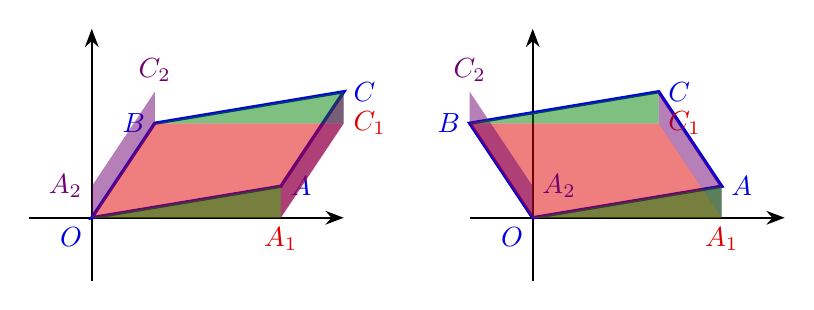
\begin{tikzpicture}[scale=.8]
		\begin{scope}
			\draw[cstaxis] (-1,0)--(4,0);
			\draw[cstaxis] (0,-1)--(0,3);
			\draw[cstcurve,main] (0,0)--(3,0.5)--(4,2)--(1,1.5)--cycle;
			\draw (0,0) node[main,below left] {$O$};
			\draw (3,0.5) node[main,right] {$A$};
			\draw (1,1.5) node[main,left]{$B$};
			\draw (4,2) node[main,right] {$C$};
			\fill[cstcurve,second,fill opacity=.5,visible on=<5->] (0,0)--(3,0)--(4,1.5)--(1,1.5)--cycle;
			\begin{scope}[visible on=<5->]
				\draw (3,0) node[second,below] {$A_1$};
				\draw (4,1.5) node[second,right] {$C_1$};
			\end{scope}
			\fill[cstcurve,third,fill opacity=.5,visible on=<6->] (0,0)--(0,0.5)--(1,2)--(1,1.5)--cycle;
			\begin{scope}[visible on=<6->]
				\draw (0,.5) node[third,left] {$A_2$};
				\draw (1,2) node[third,above] {$C_2$};
			\end{scope}
			\fill[cstcurve,fourth,fill opacity=.5,visible on=<8->] (1,1.5)--(4,1.5)--(4,2)--cycle;
			\fill[cstcurve,fourth,fill opacity=.5,visible on=<9->] (0,0)--(3,0)--(3,0.5)--cycle;
			\fill[cstcurve,third,fill opacity=.5,visible on=<10->] (3,0)--(3,0.5)--(4,2)--(4,1.5)--cycle;
		\end{scope}

		\begin{scope}[xshift=7cm,visible on=<11->]
			\draw[cstaxis] (-1,0)--(4,0);
			\draw[cstaxis] (0,-1)--(0,3);
			\draw[cstcurve,main] (0,0)--(3,0.5)--(2,2)--(-1,1.5)--cycle;
			\draw (0,0) node[main,below left] {$O$};
			\draw (3,0.5) node[main,right] {$A$};
			\draw (-1,1.5) node[main,left]{$B$};
			\draw (2,2) node[main,right] {$C$};
			\fill[cstcurve,second,fill opacity=.5,visible on=<12->] (0,0)--(3,0)--(2,1.5)--(-1,1.5)--cycle;
			\fill[cstcurve,third,fill opacity=.5,visible on=<12->] (0,0)--(0,0.5)--(-1,2)--(-1,1.5)--cycle;
			\begin{scope}[visible on=<12->]
				\draw (3,0) node[second,below] {$A_1$};
				\draw (2,1.5) node[second,right] {$C_1$};
				\draw (0,.5) node[third,right] {$A_2$};
				\draw (-1,2) node[third,above] {$C_2$};
			\end{scope}
			\fill[cstcurve,third,fill opacity=.5,visible on=<13->] (3,0)--(3,0.5)--(2,2)--(2,1.5)--cycle;
			\fill[cstcurve,fourth,fill opacity=.5,visible on=<13->] (0,0)--(3,0)--(3,0.5)--cycle;
			\fill[cstcurve,fourth,fill opacity=.5,visible on=<14->] (-1,1.5)--(2,1.5)--(2,2)--cycle;
		\end{scope}
	\end{tikzpicture}
	\end{center}
	\onslide<+->
	令 $A_1(a,0)$, 并作 $\parallelogram OA_1C_1B$;
	\onslide<+->
	令 $A_2(0,b)$, 并作 $\parallelogram OA_2C_2B$.
	\onslide<+->
	那么 $\parallelogram OACB$ 的面积是这两个相加还是相减?
	\onslide<+->\onslide<+->\onslide<+->
	使用割补法可知为\alert{二者相减}.
	
	\onslide<+->
	如果 $A$ 在第一象限, $B$ 在第二象限.
	\onslide<+->
	那么 $\parallelogram OACB$ 的面积是这两个相加还是相减?\onslide<+->\onslide<+->
	使用割补法可知为\alert{二者相加}.
\end{frame}


\begin{frame}{有向面积\noexer}
	\onslide<+->
	为何第一种情形是相减而第二种情形是相加呢?
	\onslide<+->
	观察发现: 这些平行四边形中只有第一种情形的 $\parallelogram OA_2C_2B$, 从 $OA_2$ 到 $OB$ 是顺时针方向.
	\onslide<+->
	如果定义\emph{有向面积}并记为
	\[|\bfu,\bfv|=\begin{vmatrix}
		a&c\\b&d
	\end{vmatrix}=\begin{cases}
		S_{\parallelogram OACB},&\text{从 $OA$ 到 $OB$ 是逆时针};\\
		-S_{\parallelogram OACB},&\text{从 $OA$ 到 $OB$ 是顺时针}.
	\end{cases}\]
	\onslide<+->
	那么
	\[\begin{vmatrix}
		a&c\\b&d
	\end{vmatrix}=\begin{vmatrix}
		a&c\\0&d
	\end{vmatrix}+\begin{vmatrix}
		0&c\\b&d
	\end{vmatrix}=a\begin{vmatrix}
		1&c\\0&d
	\end{vmatrix}+b\begin{vmatrix}
		0&c\\1&d
	\end{vmatrix}.\]
	\onslide<+->
	换言之, $\bfv$ 固定时, 则 $|\bfu,\bfv|$ 关于 $\bfu$ 是线性的.
	\onslide<+->
	同理, $\bfu$ 固定时, $|\bfu,\bfv|$ 关于 $\bfv$ 也是线性的.
\end{frame}


\begin{frame}{平行多面体情形\noexer}
	\onslide<+->
	将上述概念推广到 $n$ 维情形.
	\onslide<+->
	考虑 $n$ 维空间中由从原点出发的向量 $\bfv_1,\dots,\bfv_n$ 张成的平行多面体.
	\onslide<+->
	如果 $\bfv_1,\dots,\bfv_n$ 就是按顺序各个分量上的单位向量
	\[\bfe_1=(1,0,\dots,0)^\rmT,\quad
	\bfe_2=(0,1,\dots,0)^\rmT,\quad\cdots,\quad
	\bfe_n=(0,0,\dots,1)^\rmT,\]
	则有向面积为 $1$.
	\onslide<+->
	如果交换 $\bfv_i,\bfv_j$ 的位置, 有向面积相差 $-1$ 倍.
	\onslide<+->
	于是得到 $n$ 维情形的有向面积 $|\bfv_1,\dots,\bfv_n|$ 应当满足:
	\begin{enumerate}
		\item $|\bfe_1,\dots,\bfe_n|=1$;
		\item 反对称性: $|\cdots,\bfv_i,\cdots,\bfv_j,\cdots|=-|\cdots,\bfv_j,\cdots,\bfv_i,\cdots|$;
		\item $|\cdots,k\bma,\cdots|=k|\cdots,\bma,\cdots|$;
		\item $|\cdots,\bma+\bmb,\cdots|=|\cdots,\bma,\cdots|+|\cdots,\bmb,\cdots|$.
	\end{enumerate}
\end{frame}


\begin{frame}{行列式的定义\noexer}
	\onslide<+->
	设 $n$ 阶方阵 $\bfA=(a_{ij})$ 的各列形成的向量为 $\bfv_1,\dots,\bfv_n$,
	\onslide<+->
	称有向面积 $|\bfv_1,\cdots,\bfv_n|$ 就是方阵 $\bfA$ 的\emph{行列式}.
	\onslide<+->
	注意到
	\[\bfv_j=a_{1j}\bfe_1+a_{2j}\bfe_2+\cdots+a_{nj}\bfe_n,\]
	\onslide<+->
	利用线性性质将行列式展开将会得到 $n^n$ 项
	\[\sum_{k_1,k_2,\dots,k_n=1}^n|\bfe_{k_1},\cdots,\bfe_{k_n}| a_{k_11}a_{k_22}\cdots a_{k_nn}.\]

	\onslide<+->
	如果 $k_i=k_j$, 则交换 $\bfe_{k_i},\bfe_{k_j}$ 可知 $|\bfe_{k_1},\cdots,\bfe_{k_n}|=0$.
	\onslide<+->
	从而只剩下 $k_1,k_2,\dots,k_n$ 是 $1,2,\dots,n$ 的排列时的那些项.
	\onslide<+->
	例如: 
	\begin{align*}
		\begin{vmatrix}
			a_{11}&a_{12}\\
			a_{21}&a_{22}
		\end{vmatrix}&=|a_{11}\bfe_1,a_{12}\bfe_1+a_{22}\bfe_2|+|a_{21}\bfe_2,a_{12}\bfe_1+a_{22}\bfe_2|\\
		&=a_{11}a_{12}|\bfe_1,\bfe_1|+a_{11}a_{22}|\bfe_1,\bfe_2|+a_{21}a_{12}|\bfe_2,\bfe_1|+a_{21}a_{22}|\bfe_2,\bfe_2|\\
		&=a_{11}a_{22}-a_{21}a_{12}.
	\end{align*}
\end{frame}
	
	
\begin{frame}{行列式的展开形式\noexer}
	\onslide<+->
	设 $k_1,k_2,\dots,k_n$ 是 $1,2,\dots,n$ 的排列.
	\onslide<+->
	如果排列 $k_1,k_2,\dots,k_n$ 需要奇数次对换变成 $1,2,\dots,n$, 记 	$\sgn(k_1,\dots,k_n)=-1$; 否则 $\sgn(k_1,\dots,k_n)=+1$.
	\onslide<+->
	根据反对称性,
	\[|\bfe_{k_1},\cdots,\bfe_{k_n}|=\sgn(k_1,\dots,k_n)|\bfe_1,\cdots,\bfe_n|=\sgn(k_1,\dots,k_n).\]
	\onslide<+->
	\begin{definition}
		设 $\bfA=(a_{ij})$ 是 $n$ 阶方阵.
		定义 $\bfA$ 的\emph{行列式}为
		\[|\bfA|=\sum \sgn(k_1,\dots,k_n) a_{k_11}a_{k_22}\cdots a_{k_nn},\]
		其中 $k_1,k_2,\dots,k_n$ 取遍 $1,2,\dots,n$ 的全体排列.
	\end{definition}
\end{frame}


\begin{frame}{$2,3$ 阶行列式}
	\onslide<+->
	当 $n=2$ 时, $\sgn(12)=1,\sgn(21)=-1$,
	\onslide<+->
	于是
	\[\begin{vNiceMatrix}
		a_{11}&a_{12}\\
		a_{21}&a_{22}
		\CodeAfter
		\tikz \draw[thick,main,visible on=<3->] (1-|1) -- (3-|3);
		\tikz \draw[cstdash,second,visible on=<3->] (3-|1) -- (1-|3);
	\end{vNiceMatrix}
	:=a_{11}a_{22}-a_{12}a_{21}.\]

	\onslide<+->
	\onslide<+->
	当 $n=3$ 时,
	\[\sgn(123)=\sgn(231)=\sgn(312)=1,\]
	\[\sgn(132)=\sgn(213)=\sgn(321)=-1,\]
	\onslide<+->
	于是
	\[\begin{vNiceMatrix}
		a_{11}&a_{12}&a_{13}\\
		a_{21}&a_{22}&a_{23}\\
		a_{31}&a_{32}&a_{33}
		\CodeAfter
		\tikz \draw[thick,main,visible on=<6-8>] (1-|1) -- (4-|4);
		\tikz \draw[thick,second,visible on=<7-8>] (1-|2) -- (3-|4);
		\tikz \draw[thick,second,visible on=<7-8>] (3-|1) -- (4-|2);
		\tikz \draw[thick,third,visible on=<8>] (1-|3) -- (2-|4);
		\tikz \draw[thick,third,visible on=<8>] (2-|1) -- (4-|3);
		\tikz \draw[cstdash,main,visible on=<9->] (1-|4) -- (4-|1);
		\tikz \draw[cstdash,second,visible on=<10->] (1-|3) -- (3-|1);
		\tikz \draw[cstdash,second,visible on=<10->] (3-|4) -- (4-|3);
		\tikz \draw[cstdash,third,visible on=<11->] (1-|2) -- (2-|1);
		\tikz \draw[cstdash,third,visible on=<11->] (2-|4) -- (4-|2);
	\end{vNiceMatrix}
	:=
	a_{11}a_{22}a_{33}+a_{12}a_{23}a_{31}+a_{13}a_{21}a_{32}
	-a_{11}a_{23}a_{32}-a_{12}a_{21}a_{33}-a_{13}a_{22}a_{31}.
	\]
\end{frame}


\begin{frame}{例: $2,3$ 阶行列式的计算}
	\onslide<+->
	\begin{example}
		\begin{align*}
			\begin{vmatrix}
				1&3&2\\3&-5&1\\2&1&4
			\end{vmatrix}
			&\onslide<+->{=1\cdot (-5)\cdot 4+3\cdot 1\cdot2+2\cdot3\cdot1-1\cdot1\cdot1-3\cdot3\cdot4-2\cdot(-5)\cdot2}\\
			&\onslide<+->{=-20+6+6-1-36+20=-25.}
		\end{align*}
	\end{example}
	\onslide<+->
	\begin{exercise}
		若 $k>0$ 且 $\begin{vmatrix}
			k&2&1\\2&k&1\\k&1&2
		\end{vmatrix}=0$, 则 $k=$\fillblankframe{$2$}.
	\end{exercise}
\end{frame}


\begin{frame}{注记}
	\begin{enumerate}
		\item 行列式将一个方阵映射到一个数.
		\item $1$ 阶行列式就是方阵里面唯一的那个元素, 尽管也记作 $|\cdot|$, 但注意和绝对值区分.
		\item $2,3$ 阶行列式可以用对角线法直接得到展开式, 但是更高阶的没有这种表示方法.
		\item \emph{对角阵}的行列式
		\[\bigl|\diag(a_1,a_2,\dots,a_n)\bigr|=a_1a_2\cdots a_n,\]
		特别地 $|\bfE_n|=1,|\bfO_n|=0$.
		\item $|\bfA|$ 是由一些 $\pm a_{k_11}a_{k_22}\cdots a_{k_nn}$ 相加得到, 其中 $k_1,k_2,\dots,k_n$ 取遍 $1,2,\dots,n$ 的所有排列, 一共有 $n!$ 个这样的项, 其中一半取 $+$, 一半取 $-$ ($n\ge2$).
		\item {\itshape $|\bfA|$ 对应的线性变换(常数倍)是 $\bfA$ 对应的线性变换 $\BR^n\ra\BR^n$ 诱导的 $n$ 次外代数上的线性变换 $\bigwedge^n\BR^n\to\bigwedge^n\BR^n$, 感兴趣的可自行阅读有关材料.}
	\end{enumerate}
\end{frame}


% \begin{frame}{三阶行列式的几何意义}
% 	\onslide<+->
% 	类似地, 若 $A(a_1,a_2,a_3),B(b_1,b_2,b_3),C(c_1,c_2,c_3)$,
% 	\onslide<+->
% 	则三阶行列式 $\begin{vmatrix}
% 		a_1&a_2&a_3\\b_1&b_2&b_3\\c_1&c_2&c_3
% 	\end{vmatrix}$ 的绝对值就是下述平行六面体的体积.
% 	\begin{center}
% 	\begin{tikzpicture}[scale=.8]
% 		\draw[cstcurve,main] (0,0)--(3,0)--(4,1.5)--(1,1.5)--cycle;
% 		\draw[cstcurve,main] (4.5,1)--(5.5,2.5)--(2.5,2.5);
% 		\draw[cstdash,cstcurve,main] (2.5,2.5)--(1.5,1)--(4.5,1);
% 		\draw[cstdash,cstcurve,main] (0,0)--(1.5,1);
% 		\draw[cstcurve,main] (3,0)--(4.5,1);
% 		\draw[cstcurve,main] (4,1.5)--(5.5,2.5);
% 		\draw[cstcurve,main] (1,1.5)--(2.5,2.5);
% 		\draw (0,0) node[second,left] {$O$};
% 		\draw (3,0) node[second,right] {$A$};
% 		\draw (1,1.5) node[second,left] {$C$};
% 		\draw (1.5,1) node[second,below] {$B$};
% 	\end{tikzpicture}
% 	\end{center}
% 	\onslide<+->
% 	它的符号则表示使用右手四指从 $OA$ 旋转到 $OB$ 方向时, 大拇指所指方向与 $OC$ 是否在平面 $OAB$ 的同侧.
% \end{frame}


\subsection{行列式的性质}

\begin{frame}{行列式的乘性}
	\onslide<+->
	\begin{theorem@}
		\begin{enumerate}
			\item $|\bfA\bfB|=|\bfA|\cdot|\bfB|$.
		\end{enumerate}
	\end{theorem@}
	\onslide<+->
	\begin{proof}
		设 $f(\bfX):=|\bfA\bfX|$, 即 $f(\bfv_1,\dots,\bfv_n)=|\bfA\bfv_1,\dots,\bfA\bfv_n|$.
	\onslide<+->{%
			容易知道 $f$ 也满足反对称性, 且对任意 $\bfv_i$ 是线性的.
		}\onslide<+->{%
			类似于行列式展开可知, 对于 $\bfX=(a_{ij})$,
			\begin{align*}
				f(\bfX)&=\sum f(\bfe_{k_1},\dots,\bfe_{k_n})a_{k_11}a_{k_22}\cdots a_{k_nn}\\
				&=\sum f(\bfe_1,\dots,\bfe_n)\sgn(k_1,\dots,k_n)a_{k_11}a_{k_22}\cdots a_{k_nn}\\
				&=f(\bfE)|\bfX|=|\bfA|\cdot|\bfX|,
			\end{align*}
			其中 $k_1,k_2,\dots,k_n$ 取遍 $1,2,\dots,n$ 的全体排列.
		}\onslide<+->{%
			故 $|\bfA\bfB|=f(\bfB)=|\bfA|\cdot|\bfB|$.
		}
	\end{proof}
	\onslide<+->
	由此可知, 对于平行多面体 $V\subset \BR^n$, $\bfA$ 对应的线性映射将其面积变为 $|\bfA|$ 倍.
\end{frame}


\begin{frame}{例: 行列式的乘性}
	\onslide<+->
	\begin{example}
		证明:
		$\begin{vmatrix}
			a_1+b_1&b_1+c_1&c_1+a_1\\
			a_2+b_2&b_2+c_2&c_2+a_2\\
			a_3+b_3&b_3+c_3&c_3+a_3
		\end{vmatrix}=2\begin{vmatrix}
			a_1&b_1&c_1\\
			a_2&b_2&c_2\\
			a_3&b_3&c_3
		\end{vmatrix}$.
	\end{example}
	\onslide<+->
	\begin{proof}
		\[\begin{vmatrix}
			a_1+b_1&b_1+c_1&c_1+a_1\\
			a_2+b_2&b_2+c_2&c_2+a_2\\
			a_3+b_3&b_3+c_3&c_3+a_3
		\end{vmatrix}=\begin{vmatrix}
			a_1&b_1&c_1\\
			a_2&b_2&c_2\\
			a_3&b_3&c_3
		\end{vmatrix}\cdot\begin{vmatrix}
			1&0&1\\
			1&1&0\\
			0&1&1
		\end{vmatrix}\onslide<+->{=2\begin{vmatrix}
			a_1&b_1&c_1\\
			a_2&b_2&c_2\\
			a_3&b_3&c_3
		\end{vmatrix}.}\qedhere\]
	\end{proof}
\end{frame}


\begin{frame}{行列式的转置不变性}
	\onslide<+->
	\begin{theorem@}
		\begin{enumerate}
			\setcounter{enumi}{1}
			\item 转置不改变行列式: $|\bfA^\rmT|=|\bfA|$.
		\end{enumerate}
	\end{theorem@}
	\onslide<+->
	一个排列 $k_1,\dots,k_n$ 可以看成是集合 $\{1,2,\dots,n\}$ 到自身的双射 $i\mapsto k_i$.
	\onslide<+->
	设它的逆映射对应的排列是 $\ell_1,\dots,\ell_n$, 则 $\ell_{k_i}=i$.
	\onslide<+->
	由于
	\begin{align*}
		|\bfA|&=\sum\sgn(k_1,\dots,k_n) a_{k_11}\cdots a_{k_nn}=\sum\sgn(k_1,\dots,k_n)a_{1\ell_1}\cdots a_{n\ell_n},\\
		|\bfA^\rmT|&=\sum\sgn(\ell_1,\dots,\ell_n)a_{1\ell_1}\cdots a_{n\ell_n},
	\end{align*}
	\onslide<+->
	我们只需说明 $\sgn(k_1,\dots,k_n)=\sgn(\ell_1,\dots,\ell_n)$.
	\onslide<+->
	设
	\[\bfP=(\bfe_{k_1},\bfe_{k_2},\dots,\bfe_{k_n})\]
	的 $k_i$ 行 $i$ 列为 $1$, 其余项为零.
	\onslide<+->
	那么 $|\bfP|=\sgn(k_1,\dots,k_n)$, $|\bfP^\rmT|=\sgn(\ell_1,\dots,\ell_n)$.
	\onslide<+->
	由于 $\bfP\bfP^\rmT=\bfE$, 因此 $|\bfP|\cdot|\bfP^\rmT|=|\bfE|=1$.
	\onslide<+->
	而 $|\bfP|=\pm1$, 因此 $|\bfP|=|\bfP^\rmT|$.
\end{frame}


\begin{frame}{例: 方阵的行列式}
	\beqskip{6pt}
		\onslide<+->
		\begin{example}
			设 $\bfA=\begin{pmatrix}
				a&-b&-c&-d\\
				b&a&-d&c\\
				c&d&a&-b\\
				d&-c&b&a
			\end{pmatrix}$, 求 $|\bfA|$.
		\end{example}
		\onslide<+->
		\begin{solution}
			这题可以直接硬算, 不过我们可以利用一点小技巧:
		\onslide<+->{%
				\[\bfA\bfA^\rmT=\begin{pmatrix}
					a&-b&-c&-d\\
					b&a&-d&c\\
					c&d&a&-b\\
					d&-c&b&a
				\end{pmatrix}\begin{pmatrix}
					a&b&c&d\\
					-b&a&d&-c\\
					-c&-d&a&b\\
					-d&c&-b&a
				\end{pmatrix}=(a^2+b^2+c^2+d^2)\bfE.\]
			}\onslide<+->{%
				因此 $|\bfA|=\pm(a^2+b^2+c^2+d^2)^2$.
			}\onslide<+->{%
				因为 $|\bfA|$ 一定有 $a^4$ 项, 所以 $|\bfA|=(a^2+b^2+c^2+d^2)^2$.
			}
		\end{solution}
	\endgroup
\end{frame}


\begin{frame}{行列式线性性}
	\onslide<+->
	再根据行列式关于每个列向量的线性性和反对称性有:
	\onslide<+->
	\begin{theorem@}
		\begin{enumerate}
			\setcounter{enumi}{2}
			\item 互换两行(列)后, 方阵的行列式变为 $-1$ 倍.
			\item 方阵的某一行(列)乘 $k$ 后, 方阵的行列式变为 $k$ 倍.
			\item 将方阵某一行(列)对应向量写成两个向量之和, 则行列式也可对应拆成两个行列式之和.
		\end{enumerate}
	\end{theorem@}
	\onslide<+->
	\begin{corollary}
		\begin{enumerate}
			\item 具有相同的两行(列)的方阵的行列式为零: $|\cdots,\bfv,\cdots,\bfv,\cdots|=0$.
			\item 若方阵有一行(列)全为零, 则行列式为零: $|\cdots,{\bf0},\cdots|=0$.
			\item 若方阵有两行(列)成比例, 则行列式为零: $|\cdots,\bfv,\cdots,k\bfv,\cdots|=0$.
			\item 行列式中某一行(列)的公因子可以提到行列式外面.
		\end{enumerate}
	\end{corollary}
\end{frame}


\begin{frame}{初等变换}
	\onslide<+->
	计算行列式可以通过实施下列变换来化简:
	\onslide<+->
	\begin{third}{初等变换}
		\begin{enumerate}
			\item 互换两行(列): $\alertm{r_i\swap r_j, c_i\swap c_j}$, 行列式变号;
			\item 一行(列)乘\alert{非零常数} $k$: $\alertm{kr_i, kc_i}$, 行列式变为 $k$ 倍;
			\item $j$ 行(列)乘 $k$ 加到 $i$ 行(列): $\alertm{r_i+kr_j, c_i+kc_j}$, 行列式不变.
		\end{enumerate}
	\end{third}
	\onslide<+->
	实施第三类初等变换 $c_i+kc_j$ 时, 第 $j$ 列不变, 改变的是第 $i$ 列.
	\onslide<+->
	由于
	\begin{align*}
		|\cdots,\bfv_i,\cdots,\bfv_j,\cdots|
		&=|\cdots,\bfv_i,\cdots,\bfv_j,\cdots|
		+|\cdots,k\bfv_j,\cdots,\bfv_j,\cdots|\\
		&=|\cdots,\bfv_i+k\bfv_j,\cdots,\bfv_j,\cdots|,
	\end{align*}
	\onslide<+->
	因此第三类初等变换不改变行列式的值.
\end{frame}


\begin{frame}{例: 使用初等变换计算行列式}
	\onslide<+->
	\begin{exercise}
		\begin{enumerate}
			\item 判断题: $|\lambda \bfA|=\lambda|\bfA|$. \onslide<+->{\alert{$|\lambda \bfA|=\lambda^n|\bfA|$}}
			\item 判断题: $\begin{vmatrix}
				1&&&\\&2&&\\&&3&\\&&&4
			\end{vmatrix}=-\begin{vmatrix}
				&&&1\\&&2&\\&3&&\\4&&&
			\end{vmatrix}$. \onslide<+->{\alert{$|\bfe_4,\bfe_3,\bfe_2,\bfe_1|=1$}}
			\item 计算 $\begin{vmatrix}
				a_1+b_1&b_1+c_1&c_1+d_1&d_1+a_1\\
				a_2+b_2&b_2+c_2&c_2+d_2&d_2+a_2\\
				a_3+b_3&b_3+c_3&c_3+d_3&d_3+a_3\\
				a_4+b_4&b_4+c_4&c_4+d_4&d_4+a_4
			\end{vmatrix}=$\fillblankframe{$0$}.
			\item 设 $\bfA$ 为 $5$ 阶方阵, $|\bfA|=-1$, 则
				$|2\bfA|=$\fillblankframe{$-32$},
				$\bigl||\bfA|\bfA\bigr|=$\fillblankframe{$1$}.
		\end{enumerate}
	\end{exercise}
\end{frame}


\begin{frame}{例: 方阵的行列式}
	\onslide<+->
	\begin{example}
		计算
		$\begin{vmatrix}
			2\sin a\cos a&\sin a\cos b+\cos a\sin b&\sin a\cos c+\cos a\sin c\\
			\sin b\cos a+\cos b\sin a&2\sin b\cos b&\sin b\cos c+\cos b\sin c\\
			\sin c\cos a+\cos c\sin a&\sin c\cos b+\cos c\sin b&2\sin c\cos c
		\end{vmatrix}$.
	\end{example}
	\onslide<+->
	容易看出该方阵可写成两个方阵之和
	\[\begin{pmatrix}
		\sin a\cos a&\sin a\cos b&\sin a\cos c\\
		\sin b\cos a&\sin b\cos b&\sin b\cos c\\
		\sin c\cos a&\sin c\cos b&\sin c\cos c
	\end{pmatrix}+\begin{pmatrix}
		\cos a\sin a&\cos a\sin b&\cos a\sin c\\
		\cos b\sin a&\cos b\sin b&\cos b\sin c\\
		\cos c\sin a&\cos c\sin b&\cos c\sin c
	\end{pmatrix}.\]
	\onslide<+->
	这两个方阵各自满足各行成比例, 因此可分别写成
	\[\begin{pmatrix}
			\sin a\\
			\sin b\\
			\sin c
		\end{pmatrix}(\cos a,\cos b,\cos c),\qquad
		\begin{pmatrix}
			\cos a\\
			\cos b\\
			\cos c
		\end{pmatrix}(\sin a,\sin b,\sin c).\]
\end{frame}


\begin{frame}{例: 方阵的行列式}
	\onslide<+->
	因此原方阵为
	\[\begin{pmatrix}
			\sin a&\cos a\\
			\sin b&\cos b\\
			\sin c&\cos c
		\end{pmatrix}\cdot\begin{pmatrix}
			\cos a&\cos b&\cos c\\
			\sin a&\sin b&\sin c
		\end{pmatrix}.\]
	\onslide<+->
	\begin{solution}
		原式$=\begin{vmatrix}
			\sin a&\cos a&0\\
			\sin b&\cos b&0\\
			\sin c&\cos c&0
		\end{vmatrix}\cdot\begin{vmatrix}
			\cos a&\cos b&\cos c\\
			\sin a&\sin b&\sin c\\
			0&0&0
		\end{vmatrix}=0$.
	\end{solution}
	\onslide<+->
	设 $\bfA\in M_{m\times n},\bfB\in M_{n\times m}$.
	\onslide<+->
	若 $m>n$, 则
	\[\alertn{|\bfA\bfB|}=\left|
		(\bfA,\bfO_{m\times(m-n)})\begin{pmatrix}
		\bfB\\\bfO_{(m-n)\times m}
	\end{pmatrix}\right|\alertn{=0}.\]
\end{frame}


\begin{frame}{例: 方阵的行列式}
	\onslide<+->
	\begin{example}
		设 $n$ 阶方阵 $\bfA$ 是反对称阵.
		若 $n$ 是奇数, 则 $|\bfA|=0$.
	\end{example}
	\onslide<+->
	\begin{proof}
		由于 $\bfA^\rmT=-\bfA$, 于是
		\[|\bfA|=|\bfA^\rmT|=|{-\bfA}|=(-1)^n|\bfA|=-|\bfA|.\]
	\onslide<+->{%
			故 $|\bfA|=0$.\qedhere
		}
	\end{proof}
\end{frame}


\begin{frame}{例: 使用初等变换计算行列式}\small
	\onslide<+->
	\begin{example}
		若 $abcd=1$, 证明 $\bfA=\begin{pNiceMatrix}
			a^2+a^{-2}&a&a^{-1}&1\\
			b^2+b^{-2}&b&b^{-1}&1\\
			c^2+c^{-2}&c&c^{-1}&1\\
			d^2+d^{-2}&d&d^{-1}&1
		\end{pNiceMatrix}$ 行列式为零.
	\end{example}
	\onslide<+->
	\begin{proof}
		\[|\bfA|=
			\begin{vNiceMatrix}
				a^2&a&a^{-1}&1\\
				b^2&b&b^{-1}&1\\
				c^2&c&c^{-1}&1\\
				d^2&d&d^{-1}&1
			\end{vNiceMatrix}+\begin{vNiceMatrix}
				{a^{-2}}&a&a^{-1}&1\\
				{b^{-2}}&b&b^{-1}&1\\
				{c^{-2}}&c&c^{-1}&1\\
				{d^{-2}}&d&d^{-1}&1
			\end{vNiceMatrix}
			\onslide<+->{=abcd\begin{vNiceMatrix}
				a&1&{a^{-2}}&a^{-1}\\
				b&1&{b^{-2}}&b^{-1}\\
				c&1&{c^{-2}}&c^{-1}\\
				d&1&{d^{-2}}&d^{-1}
			\end{vNiceMatrix}+\begin{vNiceMatrix}
				a&{a^{-2}}&1&a^{-1}\\
				b&{b^{-2}}&1&b^{-1}\\
				c&{c^{-2}}&1&c^{-1}\\
				d&{d^{-2}}&1&d^{-1}
			\end{vNiceMatrix}.}\]
	\onslide<+->{%
			由于 $abcd=1$, 且等式右侧两个行列式相差 $-1$ 倍, 因此 $|\bfA|=0$.\qedhere
		}
	\end{proof}
\end{frame}


\subsection{拉普拉斯展开}

\begin{frame}{余子式和代数余子式}
	\onslide<+->
	我们来介绍行列式与方阵子式的联系.
	\onslide<+->
	\begin{definition}
		设 $\bfA=(a_{ij})$ 是 $n\ge2$ 阶方阵.
		\begin{enumerate}
			\item $\bfA$ 去掉第 $i$ 行和 $j$ 列得到的 $n-1$ 阶方阵的行列式称为 $\bfA$ 在 $(i,j)$ 处的\emph{余子式} (Minor), 记为 $M_{ij}$.
			\item 称 $A_{ij}=(-1)^{i+j}M_{ij}$ 为 $\bfA$ 在 $(i,j)$ 处的\emph{代数余子式} (Algebraic Minor).
		\end{enumerate}
	\end{definition}
	\onslide<+->
	注意余子式和代数余子式是数而不是矩阵.
\end{frame}


\begin{frame}{行列式与余子式的联系\noexer}
	\onslide<+->
	假设 $\bfA$ 的第 $n$ 列除了 $a_{nn}$ 都是零.
	\onslide<+->
	若 $k_n\neq n$, 则 $a_{k_11}\cdots a_{k_nn}=0$; 若 $k_n=n$, 则 $\sgn(k_1,\dots,k_{n-1},n)=\sgn(k_1,\dots,k_{n-1})$.
	\onslide<+->
	因此
	\[|\bfA|=\sum \sgn(k_1,\dots,k_{n-1},n)a_{k_1,1}\cdots a_{k_{n-1},n-1}a_{n,n}=a_{nn} M_{nn}=a_{nn} A_{nn}.\]

	\onslide<+->
	假设 $\bfA$ 的第 $j$ 列除了 $a_{ij}$ 都是零.
	\onslide<+->
	依次对 $\bfA$ 实施
	\[r_i\swap r_{i+1},\quad r_{i+1}\swap r_{i+2},\quad\dots,\quad r_{n-1}\swap r_n,\]
	得到的方阵 $\bfB$ 就是将 $\bfA$ 的第 $i$ 行移动到第 $n$ 行的后面得到的方阵.
	\onslide<+->
	由于一共 $n-i$ 次列互换, 因此 $|\bfB|=(-1)^{n-i}|\bfA|$.

	\onslide<+->
	同理, 将 $\bfB$ 的第 $j$ 列移动到第 $n$ 列的后面得到的方阵记为 $\bfC$, 则
	\[|\bfC|=(-1)^{n-j}|\bfB|=(-1)^{i+j}|\bfA|.\]
	\onslide<+->
	注意到 $\bfC$ 在 $(n,n)$ 处元素是 $a_{ij}$, 余子式是 $M_{ij}$,
	\onslide<+->
	因此
	\[|\bfC|=a_{ij}M_{ij},\qquad |\bfA|=(-1)^{i+j}a_{ij}M_{ij}=a_{ij}A_{ij}.\]
\end{frame}


\begin{frame}{行列式与余子式的联系}
	\onslide<+->
	将 $\bfA$ 的第 $j$ 列写成
	\[\begin{pmatrix}
		a_{1j}\\a_{2j}\\\vdots\\a_{nj}
	\end{pmatrix}
	=\begin{pmatrix}
		a_{1j}\\0\\\vdots\\0
	\end{pmatrix}
	+\begin{pmatrix}
		0\\a_{2j}\\\vdots\\0
	\end{pmatrix}+\cdots+\begin{pmatrix}
		0\\0\\\vdots\\a_{nj}
	\end{pmatrix},\]
	\onslide<+->
	根据行列式的线性性质, 我们得到
	\[|\bfA|=a_{1j}A_{1j}+a_{2j}A_{2j}+\cdots+a_{nj}A_{nj}.\]
	\onslide<+->
	由于转置不改变方阵的行列式, 于是得到
	\[|\bfA|=a_{i1}A_{i1}+a_{i2}A_{i2}+\cdots+a_{in}A_{in}.\]
\end{frame}


\begin{frame}{拉普拉斯展开}
	\onslide<+->
	\begin{second}{行列式沿任一行或列展开}
		方阵的行列式等于任一行(列)的元素与其对应的代数余子式乘积的和:
		\begin{align*}
			|\bfA|&=a_{i1}A_{i1}+a_{i2}A_{i2}+\cdots+a_{in}A_{in}\\
			&=a_{1j}A_{1j}+a_{2j}A_{2j}+\cdots+a_{nj}A_{nj}.
		\end{align*}
	\end{second}
	\onslide<+->
	由此也可以看出 \alert{$i\neq k$ 时,}
	\[\alertn{a_{i1}A_{k1}+a_{i2}A_{k2}+\cdots+a_{in}A_{kn}=0,}\]
	\onslide<+->
	因为它是第 $i,k$ 行相同的方阵的行列式.
\end{frame}


\begin{frame}{例: 三角阵的行列式}
	\onslide<+->
	\begin{example}
		\begin{align*}
			\begin{vmatrix}
				a_{11}&      &      &\\
				a_{21}&a_{22}&      &\\
				\vdots&\vdots&\ddots&\\
				a_{n1}&a_{n2}&\cdots&a_{nn}
			\end{vmatrix}
			&\onslide<+->{=a_{11}\begin{vmatrix}
				a_{22}&      &\\
				\vdots&\ddots&\\
				a_{n2}&\cdots&a_{nn}
			\end{vmatrix}}
			\onslide<+->{=a_{11}a_{22}\begin{vmatrix}
				a_{33}&      &\\
				\vdots&\ddots&\\
				a_{n3}&\cdots&a_{nn}
			\end{vmatrix}}\\
			&\onslide<+->{=\cdots=a_{11}a_{22}\cdots a_{nn}.}
		\end{align*}
		\onslide<+->{
			由于转置不改变行列式, 因此上\alert{三角阵行列式也等于对角元乘积}.}
	\end{example}
\end{frame}


\begin{frame}{例: 反对角阵的行列式}
	\onslide<+->
	\begin{example}
		计算 $|\bfA|$, 其中 $\bfA=\begin{pmatrix}
			&&&a_1\\&&a_2&\\&\udots&&\\a_n&&&
		\end{pmatrix}$.
	\end{example}
	\onslide<+->
	\begin{solution*}
		\begin{align*}
			|\bfA|&=(-1)^{n+1}a_1\begin{vmatrix}
				&&a_2\\&\udots&\\a_n&&
			\end{vmatrix}
			\onslide<+->{=(-1)^{n+1}a_1\cdot (-1)^{n}a_2\begin{vmatrix}
				&&a_3\\&\udots&\\a_n&&
			\end{vmatrix}}\\
			&\onslide<+->{=\cdots=\prod_{i=1}^n (-1)^{n-i}a_i}
			\onslide<+->{=(-1)^{\frac{n(n-1)}2}a_1a_2\cdots a_n.}
		\end{align*}
	\end{solution*}
\end{frame}


\begin{frame}{例: 利用初等变换计算行列式}
	\onslide<+->
	对于具体的方阵, 我们可以利用初等变换将其化为三角阵来计算行列式.
	\onslide<+->
	也可以在某一行或一列只有少数非零元时用拉普拉斯展开来降阶.
	\onslide<+->
	\begin{example}
		\begin{align*}
			\begin{vmatrix}
				2& 3& 1&-1\\
				-4&-5& 1& 3\\
				-3& 1&-5& 3\\
				1&-2& 0&-1
			\end{vmatrix}
			&\onslide<+->{\!\!\xeq[\nsmath{r_1-2r_4}]{\substack{\nsmath{r_2+4r_4}\\\nsmath{r_3+3r_4}}}\!\!
			\begin{vmatrix}
				\alertn0& 7& 1&1\\
				\alertn0&-13& 1&-1\\
				\alertn0&-5&-5&0\\
				\alertn1&-2& 0&-1
			\end{vmatrix}}
			\onslide<+->{=(-1)^{4+1}\begin{vmatrix}
				-13& 1&-1\\
				-5&-5&0\\
					7& 1&1
				\end{vmatrix}}\\
			&\onslide<+->{\xeq{\nsmath{r_3+r_1}}
			-\begin{vmatrix}
				-13& 1&\alertn{-1}\\
				-5&-5&\alertn0\\
				-6& 2&\alertn0
			\end{vmatrix}}
			\onslide<+->{=(-1)^{1+3}\begin{vmatrix}
				-5&-5\\-6&2
			\end{vmatrix}=-40.}
		\end{align*}
	\end{example}
\end{frame}


\begin{frame}{例: 利用初等变换计算行列式}
	\onslide<+->
	\begin{exercise}
		\begin{enumerate}
			\item $\begin{vmatrix}
				-2&0&1\\
				501&200&299\\
				500&200&300
			\end{vmatrix}=$\fillblankframe{$-200$}.
			\item $\begin{vmatrix}
				1&1&1\\
				a&b&c\\
				b+c&c+a&a+b
			\end{vmatrix}=$\fillblankframe{$0$}.
			\item 设 $\bma=(1,0,-1),\bfA=\bma^\rmT\bma$, 则
				$|5\bfE-\bfA^3|=$\fillblankframe{$-75$}.
		\end{enumerate}
	\end{exercise}
	\onslide<+->
	回忆: 若 $\bfA=\bma\bmb^\rmT$, 则 $\bfA^k=\lambda^{k-1}\bfA$, 其中 $k=\bmb^{\rmT}\bma$.
\end{frame}


\begin{frame}{例: 分块矩阵行列式}
	\onslide<+->
	\begin{example}
		设
		\[\bfA=\begin{pmatrix}
			a_{11}&\cdots&a_{1m}\\
			\vdots&\ddots&\vdots\\
			a_{m1}&\cdots&a_{mm}
		\end{pmatrix},\qquad
		\bfB=\begin{pmatrix}
			b_{11}&\cdots&b_{1n}\\
			\vdots&\ddots&\vdots\\
			b_{n1}&\cdots&b_{nn}
		\end{pmatrix},\]
		\[\bfC=\begin{pNiceMatrix}
			a_{11}&\cdots&a_{1m}&&&\\
			\vdots&\ddots&\vdots&&0&\\
			a_{m1}&\cdots&a_{mm}&&&\\
			*&\cdots&*&b_{11}&\cdots&b_{1n}\\
			\vdots&\ddots&\vdots&\vdots&\ddots&\vdots\\
			*&\cdots&*&b_{n1}&\cdots&b_{nn}
			\CodeAfter
			\tikz \draw[cstdash,second] (4-|1) -- (4-|7);
			\tikz \draw[cstdash,second] (1-|4) -- (7-|4);
		\end{pNiceMatrix}.\]
		证明 $|\bfC|=|\bfA|\cdot|\bfB|$.
	\end{example}
\end{frame}


\begin{frame}{例: 分块矩阵行列式}
	\onslide<+->
	\begin{proof*}
		对 $m$ 归纳.
		\onslide<+->{当 $m=1$ 时将 $|\bfC|$ 沿第一行展开可知成立.}

	\onslide<+->{%
			假设命题对于 $m-1$ 成立.
		}\onslide<+->{%
			设 $\bfA$ 在 $(1,j)$ 处的余子式为 $M_{1j}$, $\bfC$ 在 $(1,j)$ 处的余子式为 $N_{1j}$.
		}\onslide<+->{%
			则由归纳假设 $N_{1j}=M_{1j}|\bfB|$.
		}\onslide<+->{%
			因此
			\begin{align*}
				|\bfC|&=\sum_{j=1}^m (-1)^{1+j}a_{1j}N_{1j}\\
				&=\sum_{j=1}^m (-1)^{1+j}a_{1j}M_{1j}|\bfB|
				=|\bfA|\cdot|\bfB|.\qedhere
			\end{align*}
		}
	\end{proof*}
\end{frame}


\begin{frame}{例: 拉普拉斯展开的应用}
	\onslide<+->
	\begin{example}
		设 $\bfA=\begin{pmatrix}
			3&0&4&0\\
			2&2&2&2\\
			0&-7&0&0\\
			5&3&-2&2
		\end{pmatrix}$.
		计算 $A_{41}+A_{42}+A_{43}+A_{44}$ 和 $M_{41}+M_{42}+M_{43}+M_{44}$.
	\end{example}
	\onslide<+->
	\begin{solution}
		由拉普拉斯展开可知
		\[A_{41}+A_{42}+A_{43}+A_{44}
		=\begin{vmatrix}
			3&0&4&0\\
			2&2&2&2\\
			0&-7&0&0\\
			1&1&1&1
		\end{vmatrix}=0.\]
	\end{solution}
\end{frame}


\begin{frame}{例: 拉普拉斯展开的应用}
	\onslide<+->
		\begin{solution}[续解]
			\vspace{-\baselineskip}
			\begin{align*}
				M_{41}+M_{42}+M_{43}+M_{44}
				&=-A_{41}+A_{42}-A_{43}+A_{44}
				=\begin{vmatrix}
					3&0&4&0\\
					2&2&2&2\\
					0&-7&0&0\\
					-1&1&-1&1
				\end{vmatrix}\\
				&\onslide<+->{=7\begin{vmatrix}
					3&4&0\\
					2&2&2\\
					-1&-1&1
				\end{vmatrix}=-28.}
		\end{align*}
	\end{solution}
	\onslide<+->
	\begin{exercise}
		若 $\bfA=\begin{pmatrix}
			a_1&a_2&a_3&f\\
			b_1&b_2&b_3&f\\
			c_1&c_2&c_3&f\\
			d_1&d_2&d_3&f
		\end{pmatrix}$,
		则 $A_{11}+A_{21}+A_{31}+A_{41}=$\fillblankframe{$0$}.
		\vspace{-.2\baselineskip}
	\end{exercise}
\end{frame}


\subsection{行列式的计算举例}


\begin{frame}{例: 行和为常数的行列式}
	\onslide<+->
	计算 $n$ 阶矩阵的行列式可以使用初等变换将其变为三角型, 也可以使用拉普拉斯展开来对其实施降阶.
	\onslide<+->
	\begin{example}
		\begin{align*}
			\begin{vmatrix}
				a&1&\cdots&1\\
				1&a&\cdots&1\\
				\vdots&\vdots&\ddots&\vdots\\
				1&1&\cdots&a
			\end{vmatrix}
		&\onslide<+->{\xeq[\nsmath{i\ge2}]{\nsmath{c_1+c_i}}\begin{vmatrix}
				a+n-1&1&\cdots&1\\
				a+n-1&a&\cdots&1\\
				\vdots&\vdots&\ddots&\vdots\\
				a+n-1&1&\cdots&a
			\end{vmatrix}}
		\onslide<+->{=(a+n-1)\begin{vmatrix}
				1&1&\cdots&1\\
				1&a&\cdots&1\\
				\vdots&\vdots&\ddots&\vdots\\
				1&1&\cdots&a
			\end{vmatrix}}\\
		&\onslide<+->{\xeq[\nsmath{i\ge2}]{\nsmath{r_i-r_1}}(a+n-1)\begin{vmatrix}
				1&1&\cdots&1\\
				0&a-1&\cdots&0\\
				\vdots&\vdots&\ddots&\vdots\\
				0&0&\cdots&a-1
			\end{vmatrix}}
		\onslide<+->{=(a+n-1)(a-1)^{n-1}.}
		\end{align*}
	\end{example}
\end{frame}


\begin{frame}{例: 行和为常数的行列式}
	\onslide<+->
	若方阵的每行(列)之和为常数, 可用此法化简.
	\onslide<+->
	\begin{exercise}
		计算 $n$ 阶行列式 $\begin{vmatrix}
			1+a_1&a_2&\cdots&a_n\\
			a_1&1+a_2&\cdots&a_n\\
			\vdots&\vdots&\ddots&\vdots\\
			a_1&a_2&\cdots&1+a_n
		\end{vmatrix}=$\fillblankframe[4cm]{$1+a_1+\cdots+a_n$}.
	\end{exercise}
\end{frame}


\begin{frame}{例: 箭形行列式}
	\onslide<+->
	\begin{example}
		\[\begin{vmatrix}
			1&1&\cdots&1\\
			1&2&\cdots&0\\
			\vdots&\vdots&\ddots&\vdots\\
			1&0&\cdots&n
		\end{vmatrix}\onslide<+->{\xeq[\nsmath{i\ge 2}]{\nsmath{c_1-\dfrac1i c_i}}
		\begin{vmatrix}
			1-\dfrac12-\cdots-\dfrac1n&1&\cdots&1\\
			0&2&\cdots&0\\
			\vdots&\vdots&\ddots&\vdots\\
			0&0&\cdots&n
		\end{vmatrix}}
		\onslide<+->{=\Bigl(1-\frac12-\cdots-\frac1n\Bigr)n!.}\]
	\end{example}
	\onslide<+->
	一般的箭形行列式均可用此法处理.
\end{frame}


\begin{frame}{例: 特殊形状行列式}\small
	\beqskip{0pt}
	\onslide<+->
	\begin{exercise}
		计算 $n$ 阶行列式 $\begin{vmatrix}
			1&2&3&\cdots&n-1&n\\
			-1&0&3&\cdots&n-1&n\\
			-1&-2&0&\cdots&n-1&n\\
			\vdots&\vdots&\vdots&\ddots&\vdots&\vdots\\
			-1&-2&-3&\cdots&0&n\\
			-1&-2&-3&\cdots&-(n-1)&0
		\end{vmatrix}=$\fillblankframe{$n!$}.
	\end{exercise}
	\onslide<+->
	\begin{answer}
		对该方阵实施 $r_i+r_1,i\ge 2$ 即可化为上三角阵.
	\end{answer}
	\endgroup
\end{frame}


\begin{frame}{例: 降阶法}
	\beqskip{3pt}
	\onslide<+->
	\begin{example}
		计算矩阵 $\bfA_n=\begin{pmatrix}
			   x   &   -1    &    0    &\cdots&   0  &   0  \\
			   0   &    x    &   -1    &\cdots&   0  &   0  \\
			   0   &    0    &    x    &\cdots&   0  &   0  \\
			\vdots &  \vdots & \vdots  &\ddots&\vdots&\vdots\\
			   0   &    0    &    0    &\cdots&   x  &  -1  \\
				a_n  & a_{n-1} & a_{n-2} &\cdots&  a_2 & x+a_1
		\end{pmatrix}$ 的行列式.
	\end{example}
	\onslide<+->
	\begin{solution}
		沿着第一列展开得到
		\[|\bfA_n|=x|\bfA_{n-1}|+(-1)^{1+n}a_n(-1)^{n-1}=x|\bfA_{n-1}|+a_n,\]
	\onslide<+->{%
		递推或归纳可知
		\[|\bfA_n|=x(x|\bfA_{n-2}|+a_{n-1})+a_n=\cdots=x^n+a_1x^{n-1}+a_2x^{n-2}+\cdots+a_n.\]
	}\vspace{-\baselineskip}
	\end{solution}
	\endgroup
\end{frame}

\subsection{三对角和范德蒙型行列式}

\begin{frame}{例: 降阶法计算三对角矩阵行列式}
	\onslide<+->
	\begin{example}
		计算矩阵 $\bfA_n=\begin{pmatrix}
				2  &   1  &   0  &\cdots&   0  &   0  \\
				1  &   2  &   1  &\cdots&   0  &   0  \\
				0  &   1  &   2  &\cdots&   0  &   0  \\
			\vdots&\vdots&\vdots&\ddots&\vdots&\vdots\\
				0  &   0  &   0  &\cdots&   2  &   1  \\
				0  &   0  &   0  &\cdots&   1  &   2  \\
		\end{pmatrix}$ 的行列式.
	\end{example}
\end{frame}


\begin{frame}{例: 降阶法计算三对角矩阵行列式}
	\onslide<+->
	\begin{solution}
		设 $D_n=|\bfA_n|$.
	\onslide<+->{%
		沿着第一行展开得到
		\[|\bfA_n|=2|\bfA_{n-1}|-\begin{vmatrix}
			1  &   1  &   0  &\cdots&   0  &   0  \\
			0  &   2  &   1  &\cdots&   0  &   0  \\
			0  &   1  &   2  &\cdots&   0  &   0  \\
		\vdots&\vdots&\vdots&\ddots&\vdots&\vdots\\
			0  &   0  &   0  &\cdots&   2  &   1  \\
			0  &   0  &   0  &\cdots&   1  &   2
		\end{vmatrix}_{n-1}=2|\bfA_{n-1}|-|\bfA_{n-2}|,\]
	}\onslide<+->{%
		因此
		\[|\bfA_n|-|\bfA_{n-1}|=|\bfA_{n-1}|-|\bfA_{n-2}|=\cdots=|\bfA_2|-|\bfA_1|=1,\]
	}\onslide<+->{%
		从而 $|\bfA_n|=n-1+|\bfA_1|=n+1$.}
	\end{solution}
\end{frame}


\begin{frame}{例: 降阶法计算三对角矩阵行列式}
	\onslide<+->
	若主对角线元素均为 $a$, 上下副对角线元素均为 $b$ 和 $c$, 则
	\[
		|\bfA_n|-a|\bfA_{n-1}|+bc|\bfA_{n-2}|=0.
	\]
	\onslide<+->
	设 $\lambda^2-a\lambda+bc=0$ 的两个根为 $\lambda_1,\lambda_2$, 则归纳可知
	\begin{align*}
		|\bfA_n|&=\lambda_1^n+\lambda_1^{n-1}\lambda_2+\cdots+\lambda_1\lambda_2^{n-1}+\lambda_2^n\\
		&=\begin{cases}
			\dfrac{\lambda_1^{n+1}-\lambda_2^{n+1}}{\lambda_1-\lambda_2},&\text{若}\ \lambda_1\neq \lambda_2;\\[8pt]
			(n+1)\Bigl(\dfrac a2\Bigr)^n,&\text{若}\ \lambda_1=\lambda_2=\dfrac a2.
		\end{cases}
	\end{align*}
\end{frame}


\begin{frame}{例: 范德蒙行列式}
\beqskip{0pt}
	\onslide<+->
	\begin{main}{范德蒙行列式}
		设 $\bfA_n=\begin{pmatrix}
			1&1&1&\cdots&1\\
			x_1&x_2&x_3&\cdots&x_n\\
			x_1^2&x_2^2&x_3^2&\cdots&x_n^2\\
			\vdots&\vdots&\vdots&\ddots&\vdots\\
			x_1^{n-1}&x_2^{n-1}&x_3^{n-1}&\cdots&x_n^{n-1}
		\end{pmatrix}$.
		证明 \alert{$|\bfA_n|=\prod\limits_{1\le i<j\le n}(x_j-x_i)$}.
		\vspace{-.36\baselineskip}
	\end{main}
	\onslide<+->
	\begin{solution}[证明]
		归纳证明.
	\onslide<+->{%
			当 $n=1,2$ 时显然成立.
		}\onslide<+->{%
			设 $n\ge 3$, 由 $r_n-x_1 r_{n-1}, \dots,r_2-x_1r_1$ 得到
			\[|\bfA_n|=\begin{vmatrix}
				1&1&1&\cdots&1\\
				0&x_2-x_1&x_3-x_1&\cdots&x_n-x_1\\
				0&x_2(x_2-x_1)&x_3(x_3-x_1)&\cdots&x_n(x_n-x_1)\\
				\vdots&\vdots&\vdots&\ddots&\vdots\\
				0&x_2^{n-2}(x_2-x_1)&x_3^{n-2}(x_3-x_1)&\cdots&x_n^{n-2}(x_n-x_1)
			\end{vmatrix}.\]}
			\vspace{-.44\baselineskip}
	\end{solution}
\endgroup
\end{frame}


\begin{frame}{例: 范德蒙行列式}
		\onslide<+->
		\begin{proof}[续证]
		\onslide<+->{
			沿着第一列展开, 然后提取每一列的公因式 $(x_j-x_1)$ 得到
		\[|\bfA_n|
		=\prod_{j=2}^n(x_j-x_1)\begin{vmatrix}
				1&1&\cdots&1\\
				x_2&x_3&\cdots&x_n\\
				\vdots&\vdots&\ddots&\vdots\\
				x_2^{n-1}&x_3^{n-1}&\cdots&x_n^{n-1}
			\end{vmatrix}.\]}
			\onslide<+->{由归纳假设可知
			\[|\bfA_n|
		=\prod_{j=2}^n(x_j-x_1)\cdot \prod_{2\le i<j\le n}(x_j-x_i)=\prod_{1\le i<j\le n}(x_j-x_i).\qedhere\]}
	\end{proof}
\end{frame}


\begin{frame}{例: 范德蒙行列式的应用}
	\onslide<+->
	\begin{exercise}
		\begin{enumerate}
			\item $\begin{vmatrix}
				x_1^{-3}&x_2^{-3}&x_3^{-3}&x_4^{-3}\\
				x_1^{-1}&x_2^{-1}&x_3^{-1}&x_4^{-1}\\
				x_1&x_2&x_3&x_4\\
				x_1^{3}&x_2^{3}&x_3^{3}&x_4^{3}
			\end{vmatrix}=$\fillblankframe[6cm][3mm]{\onslide<+->{$x_1^{-3}x_2^{-3}x_3^{-3}x_4^{-3}\prod\limits_{1\le i<j\le 4}(x_j^2-x_i^2)$}}.
			\item $\begin{vmatrix}
				1&1&1&1\\
				1&2&3&4\\
				1&4&9&16\\
				1&8&27&65
			\end{vmatrix}=$\fillblankframe{$14$}.
			\onslide<.->{$\alert{=\begin{vmatrix}
				1&1&1&1\\
				1&2&3&4\\
				1&4&9&16\\
				1&8&27&64
			\end{vmatrix}+\begin{vmatrix}
				1&1&1&1\\
				1&2&3&4\\
				1&4&9&16\\
				0&0&0&1
			\end{vmatrix}}$}
			\item 设 $a,b,c$ 两两不等, 且 $\begin{vmatrix}
				a&b&c\\
				a^2&b^2&c^2\\
				b+c&c+a&a+b
			\end{vmatrix}=0$, 则 $a+b+c=$\fillblankframe{$0$}.
		\end{enumerate}
	\end{exercise}
\end{frame}


\begin{frame}{例: 范德蒙行列式\noexer}
	\onslide<+->
	范德蒙行列式还有另一种证明方式, 这种思路对于其它行列式的计算也有帮助.
	\onslide<+->
	\begin{proof}
		$f=|\bfA_n|$ 是 $x_1,\dots,x_n$ 的多项式, 且次数不超过 $1+2+\cdots+(n-1)$.
	\onslide<+->{%
			由于当 $x_i=x_j$ 时 $f=0$, 因此 $f$ 包含因式 $x_i-x_j$, 从而
			\[f=g\prod_{1\le i<j\le n}(x_j-x_i).\]
		}\onslide<+->{%
			比较两边次数可知 $g$ 是常数.
		}\onslide<+->{%
			注意到 $\prod\limits_{i=1}^n x_i^{i-1}$ 只出现在范德蒙行列式对角元的乘积中, 且它在 $\prod\limits_{1\le i<j\le n}(x_j-x_i)$ 中的系数是 $1$.
		}\onslide<+->{%
			因此 $g=1$.\qedhere
		}
	\end{proof}
\end{frame}


\begin{frame}{特殊形状行列式\noexer}
	% \beqskip{1pt}
	\onslide<+->
	\begin{example}
		计算 $\displaystyle\begin{vmatrix}
			1^{50}&2^{50}&\cdots&100^{50}\\
			2^{50}&3^{50}&\cdots&101^{50}\\
			\vdots&\vdots&\ddots&\vdots\\
			100^{50}&101^{50}&\cdots&199^{50}\\
		\end{vmatrix}$.
	\end{example}
	\onslide<+->
	\begin{proof}
		将第一行换成 $(x+1)^{50},\dots,(x+100)^{50}$, 并将行列式记为 $f(x)$.
	\onslide<+->{%
			那么 $f(1)=\cdots=f(99)=0$.
		}\onslide<+->{%
			注意到 $f$ 的次数不超过 $50$, 因此 $f\equiv 0$.\qedhere
		}
	\end{proof}
	\onslide<+->
	同理若 $k<n-1$, $\Bigl|\bigl((a_i+b_j)^k\bigr)_{1\le i,j\le n}\Bigr|=0$.
	% \onslide<+->
	% 对于 $k=n-1$, 可以通过
	% \[(x+b_j)^k=x^k+\rmC_k^1 x^{k-1} b_j+\cdots+\cdots+b_j^k\]
	% 将这个方阵拆分为
	% \[((a_i+b_j)^{n-1})_{ij}
	% =(a_i^{n-j})_{ij}\cdot \diag(\rmC_{n-1}^0,\rmC_{n-1}^1,\dots,\rmC_{n-1}^{n-1}) \cdot (b_j^{i-1})_{ij}.\]
	% \endgroup
\end{frame}


\begin{frame}{行列式常见计算方法总结}
	\begin{enumerate}
		\item $2,3$ 阶行列式可用对角线法直接展开.
		\item 三角阵行列式等于对角元的乘积, 分块三角阵行列式等于对角阵行列式乘积.
		\item 行列式的计算一般需要用到\alert{三类初等变换}, 创造出足够多的零.
		\item 行列式沿一行(列)的展开往往是\alert{降阶法}的必要手段.
		\item 范德蒙型行列式可处理方阵为元素幂次递增的情形.
	\end{enumerate}
\end{frame}


\section{曲线和区域}


\subsection{复数表平面曲线}


\begin{frame}{例题: 复数方程表圆}
	\onslide<+->
	很多的平面图形能用复数形式的方程来表示.
	\onslide<+->
	这种表示方程有些时候会显得更加直观和易于理解.
	\onslide<+->
	\begin{example}[sidepic,righthand width=3.3cm,indent]
		$\abs{z+2\ii}=2$.
		\onslide<+->{%
			该方程表示与 $-2\ii $ 的距离为 $2$ 的点全体, 即圆心为 $-2\ii $ 半径为 $2$ 的圆.
		}
		
		\onslide<+->{%
			一般的圆方程为 $\abs{z-z_0}=R$, 其中 $z_0$ 是圆心, $R$ 是半径.
		}
		\tcblower
		\onslide<4->{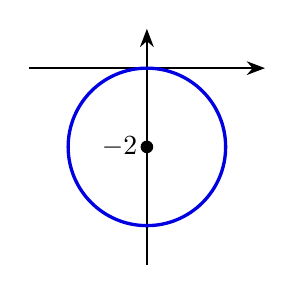
\begin{tikzpicture}
			\draw[cstaxis] (-1.5,0)--(1.5,0);
			\draw[cstaxis] (0,-2.5)--(0,.5);
			\coordinate (A) at (0,-1);
			\fill[cstdot] (A) circle
				node[left] {$-2\ii $};
			\draw[cstcurve,main] (A) circle (1);
		\end{tikzpicture}}
	\end{example}
\end{frame}


\begin{frame}{例题: 复数方程表直线}
	\onslide<+->
	\begin{example}[sidepic,righthand width=3.3cm]
		$\abs{z-4\ii}=\abs{z-2}$.
		\onslide<+->{%
			该方程表示与 $4\ii$ 和 $2$ 的距离相等的点, 即二者连线的垂直平分线.
		}\onslide<+->{%
			两边同时平方化简可得 $x-2y+3=0$.
		}\onslide<+->{%
			该方程也可以表达为
			\[
				(1+2\ii)z+(1-2\ii)\ov z+6=0.
			\]
		}
		\tcblower
		\onslide<2->{
      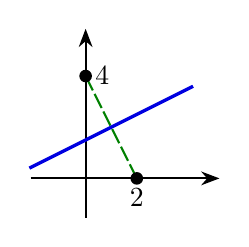
\begin{tikzpicture}[
        declare function={
          f(\y)=2*\y-1.5;
        }
      ]
        \def\u{.65}
        \draw[cstaxis] (-.7,0)--(1.7,0);
        \draw[cstaxis] (0,-.5)--(0,1.9);
        \coordinate (A) at (\u,0);
        \coordinate (B) at (0,{2*\u});
        \draw[cstdash,fourth] (A)--(B);
        \draw[cstcurve,main] ({f(.2)*\u},{.2*\u})--({f(1.8)*\u},{1.8*\u});
        \begin{scope}[cstdot]
          \fill (A) circle node[below] {$2$};
          \fill (B) circle node[right] {$4\ii$};
        \end{scope}
      \end{tikzpicture}}
	\end{example}
\end{frame}


\begin{frame}{例题: 复数方程表椭圆和双曲线}
	\onslide<+->
	\begin{example}
		$\abs{z-z_1}+\abs{z-z_2}=2a$.
		\begin{itemize}
			\item 当 $2a>\abs{z_1-z_2}$ 时, 该方程表示以 $z_1,z_2$ 为焦点, $a$ 为长半轴的椭圆;
			\item 当 $2a=\abs{z_1-z_2}$ 时, 该方程表示连接 $z_1,z_2$ 的线段;
			\item 当 $2a<\abs{z_1-z_2}$ 时, 该方程表示空集.
		\end{itemize}
	\end{example}
	\onslide<+->
	\begin{example}
		$\abs{z-z_1}-\abs{z-z_2}=2a$.
		\begin{itemize}
			\item 当 $2a<\abs{z_1-z_2}$ 时, 该方程表示以 $z_1,z_2$ 为焦点, $a$ 为实半轴的双曲线的一支;
			\item 当 $2a=\abs{z_1-z_2}$ 时, 该方程表示以 $z_2$ 为起点, 与 $z_2,z_1$ 连线反向的射线;
			\item 当 $2a>\abs{z_1-z_2}$ 时, 该方程表示空集.	
		\end{itemize}
	\end{example}
\end{frame}


\begin{frame}{例题: 复数方程表平面图形}
	\onslide<+->
	\begin{exercise}[nearnext]
		$z^2+\ov z^2=1$ 和 $z^2-\ov z^2=\ii$ 分别表示什么图形?
	\end{exercise}

	\onslide<+->
	\begin{answer}[nearprev]
		双曲线 $x^2-y^2=\dfrac12$ 和双曲线 $xy=\dfrac14$.
	\end{answer}
\end{frame}


\begin{frame}{连续曲线、闭路}
	\onslide<+->
	设 $x(t),y(t),t\in[a,b]$ 是两个连续函数.
	\onslide<+->
	参变量方程 $\begin{cases}
		x=x(t),& \\y=y(t),&
	\end{cases}t\in[a,b]$ 定义了一条\emph{连续曲线}.
	\onslide<+->
	这也等价于 $C:z=z(t)=x(t)+\ii y(t),t\in[a,b]$.
	\begin{itemize}
		\item 若除了两个端点有可能重叠外, 其它情形不会出现重叠的点, 则称 $C$ 是\emph{简单曲线}.
		\item 若连续曲线 $C$ 满足两个端点重叠, 即 $z(a) = z(b)$, 则称 $C$ 是闭合曲线.
		\item 称闭合的简单曲线为\emph{简单闭曲线}或\emph{闭路}.
	\end{itemize}
	\onslide<3->
	\begin{center}
		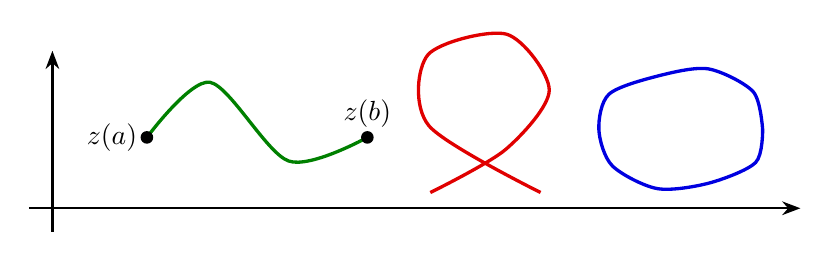
\begin{tikzpicture}
			\draw[cstaxis](-.3,.5)--(9.5,.5);
			\draw[cstaxis](0,.2)--(0,2.5);
			\coordinate (A) at (1.2,1.4);
			\coordinate (B) at (4,1.4);
			\draw[cstcurve,fourth,smooth] plot coordinates {(A) (2,2.1) (3,1.1) (B)};
			\fill[cstdot] (A) circle node[left] {$z(a)$};
			\fill[cstdot] (B) circle node[above] {$z(b)$};
			\draw[cstcurve,second,smooth,visible on=<4->] plot coordinates {(4.8,.7) (5.76,1.25) (6.31,2) (5.77,2.71) (4.77,2.45) (4.78,1.55) (6.2,.7) };
			\draw[cstcurve,main,smooth,visible on=<5->] plot coordinates {(9.02,1.5) (8.9,1.98) (8.33,2.27) (7.69,2.18) (7.07,1.95) (6.94,1.5) (7.11,1.04) (7.68,.75) (8.34,.82) (8.93,1.08) (9.02,1.5)};
		\end{tikzpicture}
	\end{center}
\end{frame}


\begin{frame}{例题: 连续曲线}
	\onslide<+->
	\begin{example}[near]
		圆 $\abs{z-z_0}=R$ 的参数方程: $z=z_0+R\ee^{\ii\theta},\quad\theta\in[0,2\pi]$.
	\end{example}
	\onslide<+->
	\begin{example}[sidepic,righthand width=150pt,near]
		直线段:
		\[
			z(t)=z_0+(z_1-z_0)t,\quad t\in[0,1],
		\]
		其中 $z_0,z_1$ 为两个端点.
		它是简单曲线.
		\tcblower
		\begin{center}
			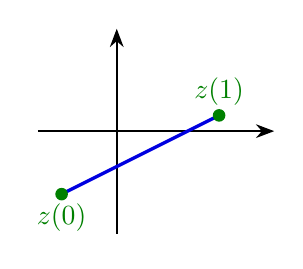
\begin{tikzpicture}
				\draw[cstaxis] (-1.3,.3)--(1.7,.3);
				\draw[cstaxis] (-.3,-1)--(-.3,1.6);
				\coordinate (A) at (-1,-.5);
				\coordinate (B) at (1,.5);
				\draw[cstcurve,main] (A)--(B);
				\begin{scope}[cstdot,fourth]
					\fill (A) circle node[below] {$z(0)$};
					\fill (B) circle node[above] {$z(1)$};
				\end{scope}
			\end{tikzpicture}
		\end{center}
	\end{example}
	\onslide<+->
	\begin{example}[sidepic,righthand width=150pt,near]
		正弦函数曲线段
		\[
			z(t)=\sin t,\quad t\in[0,2\pi]
		\]
		是简单曲线.
		\tcblower
		\begin{center}
			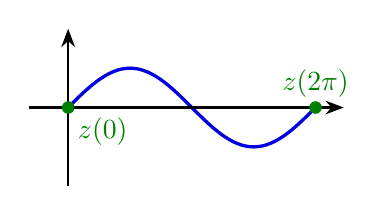
\begin{tikzpicture}
				\draw[cstcurve,main,domain=0:360,smooth] plot ({\x*pi/360},{sin(\x)*.5});
				\draw[cstaxis] (0,-1)--(0,1);
				\draw[cstaxis] (-.5,0)--(3.5,0);
				\coordinate (C) at (0,0);
				\coordinate (D) at ({pi},0);
				\begin{scope}[cstdot,fourth]
					\fill (C) circle node[below right] {$z(0)$};
					\fill (D) circle node[above] {$z(2\pi)$};
				\end{scope}
			\end{tikzpicture}
		\end{center}
	\end{example}
\end{frame}


\begin{frame}{例题: 连续曲线}
	\onslide<+->
	\begin{example}[sidepic,righthand width=150pt]
		椭圆 $\abs{z-\sqrt5}+\abs{z+\sqrt5}=6$ 的参数方程: 
		\[
			z=3\cos\theta+2\ii\sin\theta,\quad \theta\in[0,2\pi].
		\]
		\tcblower
		\begin{center}
			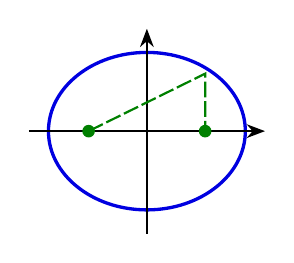
\begin{tikzpicture}
				\coordinate (E) at (-.74,0);
				\coordinate (F) at (.74,0);
				\draw[cstcurve,main] (0,0) circle(1.25 and 1);
				\draw[cstaxis] (-1.5,0)--(1.5,0);
				\draw[cstaxis] (0,-1.3)--(0,1.3);
				\draw[cstdash,fourth] (E)--(.74,.73)--(F);
				\begin{scope}[cstdot,fourth]
					\fill (E) circle;
					\fill (F) circle;
				\end{scope}
			\end{tikzpicture}
		\end{center}
	\end{example}
	\onslide<+->
	\begin{example}[sidepic,righthand width=150pt]
		双纽线 $\abs{z^2-1}=1$ 是闭合曲线, 但不是闭路.
		\tcblower
		\begin{center}
			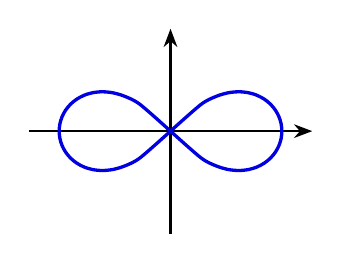
\begin{tikzpicture}
				\draw[cstaxis] (-1.8,0)--(1.8,0);
				\draw[cstaxis] (0,-1.3)--(0,1.3);
				\draw[cstcurve,main,domain=-45:45,smooth] plot ({sqrt(2*cos(2*\x))*cos(\x)},{sqrt(2*cos(2*\x))*sin(\x)});
				\draw[cstcurve,main,domain=-45:45,smooth] plot ({-sqrt(2*cos(2*\x))*cos(\x)},{sqrt(2*cos(2*\x))*sin(\x)});
			\end{tikzpicture}
		\end{center}
	\end{example}
\end{frame}


\subsection{区域和闭区域}


\begin{frame}{邻域}
	\onslide<+->
	为了引入极限的概念, 我们需要考虑点的邻域.
	\onslide<+->
	类比于高等数学中的邻域和去心邻域, 我们在复变函数中, 称开圆盘
		\[
			U(z_0,\delta)=\{z:\abs{z-z_0}<\delta\}
		\]
		为 $z_0$ 的一个 \emph{$\delta$-邻域}.
	\onslide<+->
	称去心开圆盘
		\[
			\Uc(z_0,\delta)=\{z:0<\abs{z-z_0}<\delta\}
		\]
		为 $z_0$ 的一个\emph{去心 $\delta$-邻域}.
	\onslide<2->
	\begin{center}
		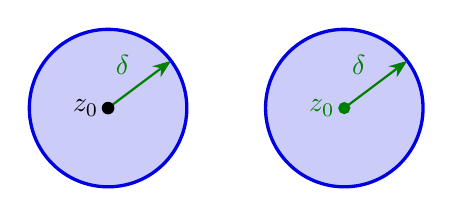
\begin{tikzpicture}
			\begin{scope}
				\coordinate (A) at (-1,0);
				\coordinate (B) at (2,0);
				\filldraw[cstcurve,main,cstfill1] (A) circle (1);
				\filldraw[cstcurve,main,cstfill1,visible on=<3->] (B) circle (1);
				\draw[cstra,fourth,thick] (A)--++(.8,.6)
					node[midway,above left] {$\delta$};
				\draw[cstra,fourth,thick,visible on=<3->] (B)--++(.8,.6)
					node[midway,above left] {$\delta$};
			\end{scope}
			\fill[cstdot] (A) circle node[left] {$z_0$};
			\filldraw[cstdote,fourth,visible on=<3->] (B) circle node[left] {$z_0$};
		\end{tikzpicture}
	\end{center}
\end{frame}


\begin{frame}{内部、外部、边界}
	\onslide<+->
	设 $G$ 是复平面的一个子集, $z_0\in\BC$.
	\onslide<+->
	它们的位置关系有三种可能:
		\begin{enumerate}
			\item 若存在 $z_0$ 的一个邻域 $U$ 完全包含在 $G$ 中, 则称 $z_0$ 是 $G$ 的一个\emph{内点}.
			\item 若存在 $z_0$ 的一个邻域 $U$ 完全不包含在 $G$ 中, 则称 $z_0$ 是 $G$ 的一个\emph{外点}.
			\item 若 $z_0$ 既不是内点也不是外点, 则称 $z_0$ 是 $G$ 的一个\emph{边界点}.
		\end{enumerate}
	\onslide<+->
	内点都属于 $G$, 外点都不属于 $G$, 而边界点则都有可能.
	\onslide<+->
	这类比于区间的端点和区间的关系.
	\onslide<1->
	\begin{center}
		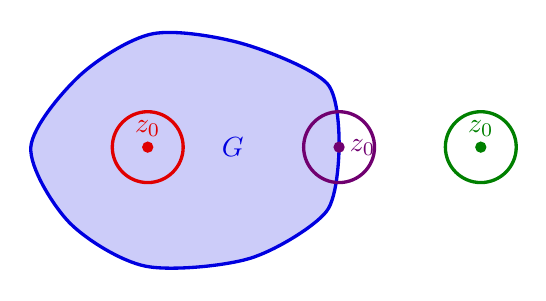
\begin{tikzpicture}[scale=.9]
			\filldraw[cstcurve,main,cstfill1,smooth] plot coordinates {(2,0) (1.83,.9) (.64,1.46) (-.63,1.6) (-1.66,1.01) (-2.35,0) (-1.81,-1.06) (-.73,-1.68) (.74,-1.57) (1.82,-.91) (2,0)};
			\begin{scope}[visible on=<3->]
				\coordinate (A) at (-.7,0);
				\draw[cstcurve,second] (A) circle (.5) node[above] {$z_0$};
				\fill[cstdot,second] (A) circle;
			\end{scope}
			\begin{scope}[visible on=<5->]
				\coordinate (B) at (2,0);
				\draw[cstcurve,third] (B) circle (.5) node[right] {$z_0$};
				\fill[cstdot,third] (B) circle;
			\end{scope}
			\begin{scope}[visible on=<4->]
				\coordinate (C) at (4,0);
				\draw[cstcurve,fourth] (C) circle (.5) node[above] {$z_0$};
				\fill[cstdot,fourth] (C) circle;
			\end{scope}
			\draw (.5,0) node[main] {$G$};
		\end{tikzpicture}
	\end{center}
\end{frame}


\begin{frame}{开集和闭集、有界和无界}
	\onslide<+->
	\begin{definition}[nearnext]
		\begin{enumerate}
			\item 若 $G$ 的所有点都是内点, 也就是说, $G$ 的边界点都不属于它, 称 $G$ 是一个\emph{开集}.
			\item 若 $G$ 的所有边界点都属于 $G$, 称 $G$ 是一个\emph{闭集}.
		\end{enumerate}
	\end{definition}
	\onslide<+->
	$G$ 是一个闭集当且仅当它的补集是开集.

	\onslide<+->
	例如
	\[
		\abs{z-z_0}<R,\quad 1<\Re z<3,\quad\frac\pi4<\arg z<\dfrac{3\pi}4
	\]
	都是开集.
	\onslide<+->
	直观上看: 开集往往由 $>,<$ 的不等式给出, 闭集往往由 $\ge,\le$ 的不等式给出. 
	\onslide<+->
	不过注意这并不是绝对的.

	\onslide<+->
	若 $D$ 可以被包含在某个开圆盘 $U(0,R)$ 中, 则称它是\emph{有界}的.
	\onslide<+->
	否则称它是\emph{无界}的.
\end{frame}


\begin{frame}{区域和闭区域}
	\onslide<+->
	\begin{definition}
		若开集 $D$ 的任意两个点之间都可以用一条完全包含在 $D$ 中的折线连接起来, 则称 $D$ 是一个\emph{区域}.
		\onslide<+->{%
			也就是说, 区域是连通的开集.
		}
	\end{definition}
	\onslide<+->
	\begin{twopart}[indent]{132pt}
		观察右侧图案, 阴影部分(不包含线条部分)中任意两点可用折线连接, 因此它是一个区域.
		\onslide<+->
		这些线条和点构成了它的边界.

		\onslide<+->
		区域和它的边界一起构成了\emph{闭区域}, 记作 $\ov D$.
		\onslide<+->
		它是一个闭集.
		\tcblower
		\onslide<3->
		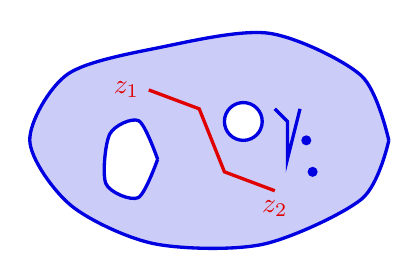
\begin{tikzpicture}[scale=.8]
			\filldraw[cstcurve,main,cstfill1,smooth] plot coordinates {(2.81,0) (2.37,1.03) (.91,1.7) (-.8,1.48) (-2.29,1.05) (-2.89,0) (-2.24,-1.03) (-.92,-1.64) (.81,-1.65) (2.38,-.93) (2.81,0)};
			\filldraw[cstcurve,main,fill=white,smooth] plot coordinates {(-.86,-.3) (-1.16,.31) (-1.62,.1) (-1.68,-.69) (-1.17,-.91) (-.86,-.3)};
			\filldraw[cstcurve,main,fill=white] (.5,.3) circle (.3);
			\fill[cstdot,main] (1.5,0) circle;
			\fill[cstdot,main] (1.6,-.5) circle;
			\draw[cstcurve,second,main] plot coordinates {(1,.5) (1.2,.3) (1.2,-.3) (1.4,.5)};
			\coordinate [label=left:\textcolor{second}{$z_1$}] (A) at (-1,.8);
			\coordinate [label=below:\textcolor{second}{$z_2$}] (B) at (1,-.8);
			\draw[cstcurve,second] (A)--(-.2,.5)--(.2,-.5)--(B);
		\end{tikzpicture}
	\end{twopart}
	\onslide<+->
	注意数学中边界的概念与日常所说的边界是两码事.
	\onslide<+->
	例如区域 $\abs{z}>1$ 的边界是 $\abs{z}=1$, 其闭区域是 $\abs{z}\ge 1$.
\end{frame}


\begin{frame}{常见区域}\small
	\onslide<+->
	很多区域可以由复数的实部、虚部、模和辐角的不等式所确定.
	\onslide<7->{%
		下方区域对应的闭区域是什么?
	}\bigdel
	\onslide<2->
	\begin{figure}[hbpt]
		\begin{minipage}{.24\textwidth}
			\centering
			\begin{tikzpicture}[scale=.7]
				\draw[cstaxis](-1.5,0)--(1.5,0);
				\draw[cstaxis](0,-1.5)--(0,1.5);
				\fill[cstfille1] (-1.2,0) rectangle (1.2,.8);
				\draw (0,-1.5) node[below,align=center] {上半平面\\$\Im z>0$};
			\end{tikzpicture}
		\end{minipage}
		\begin{minipage}{.24\textwidth}
			\centering
			\begin{tikzpicture}[scale=.7]
				\draw[cstaxis](-1.5,0)--(1.5,0);
				\draw[cstaxis](0,-1.5)--(0,1.5);
				\fill[cstfille1] (-1.2,0) rectangle (1.2,-.8);
				\draw (0,-1.5) node[below,align=center] {下半平面\\$\Im z<0$};
			\end{tikzpicture}
		\end{minipage}
		\begin{minipage}{.24\textwidth}
			\centering
			\begin{tikzpicture}[scale=.7,visible on=<3->]
				\draw[cstaxis](-1.5,0)--(1.5,0);
				\draw[cstaxis](0,-1.5)--(0,1.5);
				\fill[cstfille1] (-1.2,-1) rectangle (0,1);
				\draw (0,-1.5) node[below,align=center] {左半平面\\$\Re z<0$};
			\end{tikzpicture}
		\end{minipage}
		\begin{minipage}{.24\textwidth}
			\centering
			\begin{tikzpicture}[scale=.7,visible on=<3->]
				\draw[cstaxis](-1.5,0)--(1.5,0);
				\draw[cstaxis](0,-1.5)--(0,1.5);
				\fill[cstfille1] (0,1) rectangle (1.2,-1);
				\draw (0,-1.5) node[below,align=center] {右半平面\\$\Re z>0$};
			\end{tikzpicture}
		\end{minipage}
	\end{figure}
	\vspace{-.5\baselineskip}	
	\begin{figure}[hbpt]
		\begin{minipage}{.24\textwidth}
			\centering
			\begin{tikzpicture}[scale=.7,visible on=<4->]
				\draw[cstaxis](-1.5,0)--(1.5,0);
				\draw[cstaxis](0,-1.5)--(0,1.5);
				\fill[cstfille1] (-.6,-1) rectangle (.2,1);
				\draw[cstcurve,main] (-.6,-1)--(-.6,1);
				\draw[cstcurve,main] (.2,-1)--(.2,1);
				\draw (0,-1.5) node[below,align=center] {竖直带状区域\\$x_1<\Re z<x_2$};
			\end{tikzpicture}
		\end{minipage}
		\begin{minipage}{.24\textwidth}
			\centering
			\begin{tikzpicture}[scale=.7,visible on=<4->]
				\draw[cstaxis](-1.5,0)--(1.5,0);
				\draw[cstaxis](0,-1.5)--(0,1.5);
				\fill[cstfille1] (-1,-.4) rectangle (1,.4);
				\draw[cstcurve,main] (-1,-.4)--(1,-.4);
				\draw[cstcurve,main] (-1,.4)--(1,.4);
				\draw (0,-1.5) node[below,align=center] {水平带状区域\\$y_1<\Im z<y_2$};
			\end{tikzpicture}
		\end{minipage}
		\begin{minipage}{.24\textwidth}
			\centering
			\begin{tikzpicture}[scale=.7,visible on=<5->]
				\draw[cstaxis](-.5,0)--(2.5,0);
				\draw[cstaxis](0,-.5)--(0,2.5);
				\coordinate (A) at (0,0);
				\coordinate (B) at ({2.2*cos(60)},{2.2*sin(60)});
				\coordinate (C) at ({2.2*cos(10)},{2.2*sin(10)});
				\fill[cstfille1] (A)--(B) arc(60:10:2.2)--cycle;
				\draw[cstcurve,main] (C)--(A)--(B);
				\draw (1,-.5) node[below,align=center] {角状区域\\$\alpha_1<\arg z<\alpha_2$};
			\end{tikzpicture}
		\end{minipage}
		\begin{minipage}{.24\textwidth}
			\centering
			\begin{tikzpicture}[scale=.7,visible on=<6->]
				\filldraw[cstcurve,main,cstfill1] (0,0) circle (1.2);
				\filldraw[cstcurve,main,fill=white] (0,0) circle (.6);
				\draw[cstaxis](-1.5,0)--(1.5,0);
				\draw[cstaxis](0,-1.5)--(0,1.5);
				\draw (0,-1.5) node[below,align=center] {圆环域\\$r<\abs{z}<R$};
			\end{tikzpicture}
		\end{minipage}
	\end{figure}
\end{frame}


\subsection{区域的特性}


\begin{frame}{闭路的内部和外部}
	\onslide<+->
	闭路 $C$ 把复平面划分成了两个区域, 一个有界一个无界.
	\onslide<+->
	分别称这两个区域是 $C$ 的\emph{内部}和\emph{外部}.
	\onslide<+->
	$C$ 是它们的公共边界.
	\onslide<1->
	\begin{center}
		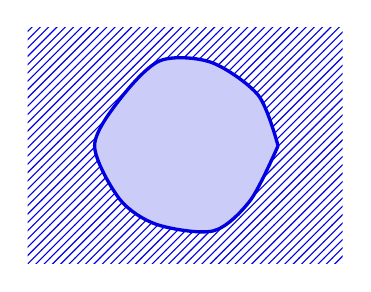
\begin{tikzpicture}
			\fill[cstfille1] (-2,-1.5) rectangle (2,1.5);
			\filldraw[cstcurve,main,cstfill1,smooth] plot coordinates {(1.18,0) (.93,.64) (.33,1.06) (-.32,1.08) (-.83,.59) (-1.15,0) (-.83,-.68) (-.36,-1) (.36,-1.08) (.83,-.69) (1.18,0)};
		\end{tikzpicture}
	\end{center}
\end{frame}


\begin{frame}{单连通区域和多连通区域}
	\onslide<+->
	在前面所说的几个常见区域的例子中, 我们在区域中画一条闭路.
	\onslide<+->
	除了圆环域之外, 闭路的内部仍然包含在这个区域内.
	\onslide<+->
	\begin{definition}
		若区域 $D$ 中的任一闭路的内部都包含在 $D$ 中, 则称 $D$ 是\emph{单连通区域}.
		否则称之为\emph{多连通区域}.
	\end{definition}
	\onslide<+->
	单连通区域内的任一闭路可以``连续地变形''成一个点.
	\onslide<+->
	这也等价于: 设 $\ell_0,\ell_1$ 是从 $A$ 到 $B$ 的两条连续曲线, 则 $\ell_0$ 可以连续地变形为 $\ell_1$ 且保持端点不动.
	\onslide<4->
	\bigdel
	\begin{center}
		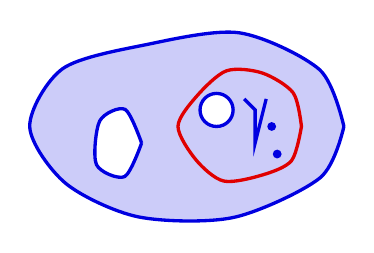
\begin{tikzpicture}[scale=.7]
			\filldraw[cstcurve,main,cstfill1,smooth] plot coordinates {(2.81,0) (2.37,1.03) (.91,1.7) (-.8,1.48) (-2.29,1.05) (-2.89,0) (-2.24,-1.03) (-.92,-1.64) (.81,-1.65) (2.38,-.93) (2.81,0)};
			\filldraw[cstcurve,main,fill=white,smooth] plot coordinates {(-.86,-.3) (-1.16,.31) (-1.62,.1) (-1.68,-.69) (-1.17,-.91) (-.86,-.3)};
			\filldraw[cstcurve,main,fill=white] (.5,.3) circle (.3);
			\fill[cstdot,main] (1.5,0) circle;
			\fill[cstdot,main] (1.6,-.5) circle;
			\draw[cstcurve,main] plot coordinates {(1,.5) (1.2,.3) (1.2,-.3) (1.4,.5)};
			\draw[cstcurve,second,smooth,visible on=<5->,shift={(.1,.2)}] plot coordinates {(1.94,-.2) (1.79,.41) (1.23,.77) (.58,.81) (.04,.35) (-.3,-.2) (.03,-.81) (.53,-1.19) (1.23,-1.08) (1.76,-.82) (1.94,-.2)};
		\end{tikzpicture}
	\end{center}
\end{frame}


\begin{frame}{典型例题: 区域的特性}
	\onslide<+->
	\begin{example}[sidepic,righthand width=3.3cm]
		$\Re(z^2)<1$.
		\onslide<+->{%
			设 $z=x+y\ii$, 则 $\Re(z^2)=x^2-y^2<1$.
		}\onslide<+->{%
			这是无界的单连通区域.
		}
		\tcblower
		\onslide<2->{%
		\begin{center}
			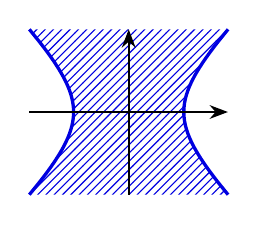
\begin{tikzpicture}[scale=.7]
				\def\t{{atan(1.5)}}
				\fill[cstfille1,domain=-\t:\t,smooth] plot ({sec(\x)},{tan(\x)})
				-- plot[domain=\t:-\t] ({-sec(\x)},{tan(\x)})
				--cycle;
				\draw[cstcurve,main,domain=-\t:\t,smooth] plot ({sec(\x)},{tan(\x)});
				\draw[cstcurve,main,domain=-\t:\t,smooth] plot ({-sec(\x)},{tan(\x)});
				\draw[cstaxis] (-1.8,0)--(1.8,0);
				\draw[cstaxis] (0,-1.5)--(0,1.5);
			\end{tikzpicture}
		\end{center}}
	\end{example}
	\onslide<+->
	\begin{example}[sidepic,righthand width=3.3cm]
		$\arg z\neq \pi$. 
		\onslide<+->{%
			即角状区域 $-\pi<\arg z<\pi$.
		}\onslide<+->{%
			这是无界的单连通区域.
		}
		\tcblower
		\onslide<5->{%
		\begin{center}
			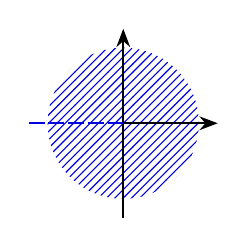
\begin{tikzpicture}[scale=.8]
				\fill[cstfille1] (0,0) circle (1.2);
				\draw[cstaxis] (0,0)--(1.5,0);
				\draw[cstaxis] (0,-1.5)--(0,1.5);
				\draw[cstdash,main] (-1.5,0)--(0,0);
			\end{tikzpicture}
		\end{center}}
	\end{example}
\end{frame}


\begin{frame}{典型例题: 区域的特性}
	\onslide<+->
	\begin{example}[near,sidepic,righthand width=3.3cm]
		$\Bigabs{\dfrac1z}\le3$.
		\onslide<+->{%
			即 $\abs{z}\ge\dfrac13$.
		}\onslide<+->{%
			这是无界的多连通\alertn{闭区域}.
		}
		\tcblower
		\onslide<2->{%
		\begin{center}
			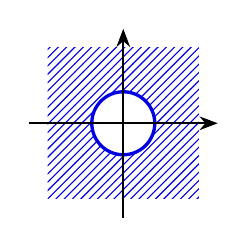
\begin{tikzpicture}[scale=.8]
				\fill[cstfille1] (-1.2,-1.2) rectangle (1.2,1.2);
				\filldraw[cstcurve,main,fill=white] (0,0) circle (.5);
				\draw[cstaxis] (-1.5,0)--(1.5,0);
				\draw[cstaxis] (0,-1.5)--(0,1.5);
			\end{tikzpicture}
		\end{center}}
	\end{example}
	\onslide<+->
	\begin{example}[near,sidepic,righthand width=3.3cm]
		$\abs{z+1}+\abs{z-1}<4$.
		\onslide<+->{%
			表示一个椭圆的内部.
		}\onslide<+->{%
			这是有界的单连通区域.
		}
		
		\tcblower
		\onslide<5->{%
		\begin{center}
			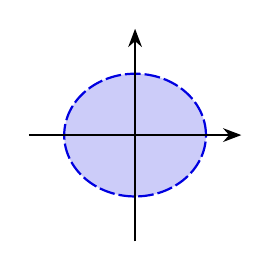
\begin{tikzpicture}[scale=.9]
				\filldraw[cstdash,main,cstfill1] (0,0) circle (1 and {0.5*sqrt(3)});
				\draw[cstaxis] (-1.5,0)--(1.5,0);
				\draw[cstaxis] (0,-1.5)--(0,1.5);
			\end{tikzpicture}
		\end{center}}
	\end{example}
	\onslide<+->
	\begin{exercise}[near]
		$\abs{z+1}+\abs{z-1}\ge 1$ 表示什么集合?
		\onslide<+->{\alertn{整个复平面.}}
	\end{exercise}
\end{frame}


\section{分块矩阵}

\subsection{分块矩阵的定义和运算}

\begin{frame}{分块矩阵的定义}
	\onslide<+->
	有时为了研究矩阵和其部分元素形成的矩阵的联系, 需要使用\emph{分块法}将其进行拆分:
	\onslide<+->
	\begin{definition}[分块矩阵]
		用若干条横线和竖线将矩阵 $\bfA$ 分成许多小矩阵, 每个小矩阵成为 $\bfA$ 的子块, 以子块为元素的矩阵称为\emph{分块矩阵}.
	\end{definition}
	\onslide<+->
	例如
	\[\bfA=\begin{pmatrix}
		\bfO_{m\times n}&\bfE_m\\
		\bfE_n&\bfO_{n\times m}
	\end{pmatrix}\]
	就是一个分块矩阵.
	\onslide<+->
	事实上我们已经不加声明地用过分块矩阵了.
\end{frame}


\begin{frame}{分块矩阵的运算: 加法和数乘}
	\onslide<+->
	若分块矩阵 $\bfA,\bfB$ 同型, 且每个对应分块也同型, 则 $\bfA+\bfB$ 就是对应分块相加形成的分块矩阵:
	\[\begin{pmatrix}
		\bfA_{11}&\cdots&\bfA_{1r}\\
		\vdots&\ddots&\vdots\\
		\bfA_{s1}&\cdots&\bfA_{sr}
	\end{pmatrix}+\begin{pmatrix}
		\bfB_{11}&\cdots&\bfB_{1r}\\
		\vdots&\ddots&\vdots\\
		\bfB_{s1}&\cdots&\bfB_{sr}
	\end{pmatrix}=\begin{pmatrix}
		\bfA_{11}+\bfB_{11}&\cdots&\bfA_{1r}+\bfB_{1r}\\
		\vdots&\ddots&\vdots\\
		\bfA_{s1}+\bfB_{s1}&\cdots&\bfA_{sr}+\bfB_{sr}
	\end{pmatrix}.\]

	\onslide<+->
	数 $\lambda$ 和分块矩阵的数乘, 就是 $\lambda$ 和对应分块数乘形成的分块矩阵:
	\[\lambda\begin{pmatrix}
		\bfA_{11}&\cdots&\bfA_{1r}\\
		\vdots&\ddots&\vdots\\
		\bfA_{s1}&\cdots&\bfA_{sr}
	\end{pmatrix}=\begin{pmatrix}
		\lambda\bfA_{11}&\cdots&\lambda\bfA_{1r}\\
		\vdots&\ddots&\vdots\\
		\lambda\bfA_{s1}&\cdots&\lambda\bfA_{sr}
	\end{pmatrix}.\]
\end{frame}


\begin{frame}{分块矩阵的运算: 乘法}
	\onslide<+->
	设
	\[\bfA=\begin{pmatrix}
		\bfA_{11}&\cdots&\bfA_{1r}\\
		\vdots&\ddots&\vdots\\
		\bfA_{s1}&\cdots&\bfA_{sr}
	\end{pmatrix},\quad
	\bfB=\begin{pmatrix}
		\bfB_{11}&\cdots&\bfB_{1t}\\
		\vdots&\ddots&\vdots\\
		\bfB_{r1}&\cdots&\bfB_{rt},
	\end{pmatrix}\]
	且 $\bfA_{ij}$ 的列数和 $\bfB_{jk}$ 的行数相同, 则
	\[\bfA\bfB=\begin{pmatrix}
		\bfC_{11}&\cdots&\bfC_{1r}\\
		\vdots&\ddots&\vdots\\
		\bfC_{s1}&\cdots&\bfC_{sr}
	\end{pmatrix},\quad\bfC_{ij}=\sum_{k=1}^r \bfA_{ik}\bfB_{kj}.\]
	\onslide<+->
	简单来说就是, 若对应的分块能做相应运算, 则分块矩阵的运算就如同把这些分块视作数一样运算.
\end{frame}


\begin{frame}{分块矩阵的运算: 转置}
	\onslide<+->
	设
	\[\bfA=\begin{pmatrix}
		\bfA_{11}&\cdots&\bfA_{1r}\\
		\vdots&\ddots&\vdots\\
		\bfA_{s1}&\cdots&\bfA_{sr}
	\end{pmatrix},\]
	则
	\[\bfA^\rmT=\begin{pmatrix}
		\bfA_{11}^\rmT&\cdots&\bfA_{s1}^\rmT\\
		\vdots&\ddots&\vdots\\
		\bfA_{1r}^\rmT&\cdots&\bfA_{sr}^\rmT
	\end{pmatrix}.\]
	\onslide<+->
	注意小块的位置需要转置, 每个小块也需要转置.
\end{frame}


\subsection{特殊分块矩阵}
\begin{frame}{分块对角阵}
	\onslide<+->
	若方阵
	\[\bfA=\begin{pmatrix}
		\bfA_1&&\\
		&\ddots&\\
		&&\bfA_m
	\end{pmatrix},\]
	其中 $\bfA_1,\dots,\bfA_m$ 都是方阵,
	\onslide<+->
	称 $\bfA$ 为\emph{分块对角阵}.
	\onslide<+->
	记作 $\bfA=\diag(\bfA_1,\dots,\bfA_m)$.

	\onslide<+->
	分块对角阵具有如下性质:
	\begin{enumerate}
		\item $|\bfA|=|\bfA_1|\cdots|\bfA_m|$;
		\item $\bfA$ 可逆当且仅当 $\bfA_1,\dots,\bfA_m$ 均可逆, 此时
		$\bfA^{-1}=\diag(\bfA_1^{-1},\dots,\bfA_m^{-1})$.
		\item $\bfA^k=\diag(\bfA_1^k,\dots,\bfA_m^k)$.
	\end{enumerate}
\end{frame}


\begin{frame}{例: 分块对角阵}
	\onslide<+->
	\begin{example}
		求 $\bfA=\begin{pmatrix}
			2&1&0&0\\
			1&1&0&0\\
			0&0&2&0\\
			0&0&-1&3
		\end{pmatrix}$ 的逆矩阵.
	\end{example}
	\onslide<+->
	\begin{solution}
		设 $\bfA_1=\begin{pmatrix}
			2&1\\1&1
		\end{pmatrix},\bfA_2=\begin{pmatrix}
			2&0\\-1&3
		\end{pmatrix}$,
		\onslide<+->{%
			则 $\bfA_1^{-1}=\begin{pmatrix}
				1&-1\\-1&2
			\end{pmatrix},\quad\bfA_2^{-1}=\dfrac16\begin{pmatrix}
				3&0\\1&2
			\end{pmatrix}$.
		}

		\onslide<+->{%
			故 $\bfA^{-1}=\diag(\bfA_1^{-1},\bfA_2^{-1})=\begin{pNiceMatrix}
				1&-1&&\\
				-1&2&&\\
				&&1/2&0\\
				&&1/6&1/3
			\end{pNiceMatrix}$.
		}
	\end{solution}
\end{frame}


\begin{frame}{例: 分块三角阵的逆}
\beqskip{2pt}
	\onslide<+->
	\begin{example}
		设 $\bfA,\bfB$ 均可逆, 求 $\begin{pmatrix}
			\bfA&\bfO\\\bfC&\bfB
		\end{pmatrix}$ 的逆矩阵.
	\end{example}
	\onslide<+->
	\begin{solution}
		由 $\begin{vmatrix}
			\bfA&\bfO\\\bfC&\bfB
		\end{vmatrix}=|\bfA|\cdot|\bfB|\neq0$ 可知该方阵可逆.
		\onslide<+->{%
			设 $\begin{pmatrix}
				\bfA&\bfO\\\bfC&\bfB
			\end{pmatrix}\begin{pmatrix}
				\bfA_1&\bfA_2\\\bfA_3&\bfA_4
			\end{pmatrix}=\bfE$.
		}
		
		\onslide<+->{%
			则 $\bfA\bfA_1=\bfE, \bfA\bfA_2=\bfO, \bfC\bfA_2+\bfB\bfA_4=\bfE$.
		}\onslide<+->{%
			于是 $\bfA_1=\bfA^{-1},\bfA_2=\bfO,\bfA_4=\bfB^{-1}$.
		}\onslide<+->{%
			再由 $\bfC\bfA_1+\bfB\bfA_3=\bfO$ 可得
			\[\bfA_3=-\bfB^{-1}\bfC\bfA_1=-\bfB^{-1}\bfC\bfA^{-1}.\]
		}\onslide<+->{%
			故 $\begin{pmatrix}
				\bfA&\bfO\\\bfC&\bfB
			\end{pmatrix}^{-1}=\begin{pmatrix}
				\bfA^{-1}&\bfO\\-\bfB^{-1}\bfC\bfA^{-1}&\bfB^{-1}
			\end{pmatrix}$.
		}
	\end{solution}
	\onslide<+->
	由此可知, (分块)上/下三角阵的逆还是(分块)上/下三角阵.
\endgroup
\end{frame}


\begin{frame}{例: 分块方阵的伴随}
	\onslide<+->
	\begin{exercise}
		设 $\bfA,\bfB$ 为同阶方阵, $\bfC=\begin{pmatrix}
			&\bfA\\\bfB&
		\end{pmatrix}$,
		则 $\bfC^*=$\fillbrace{\visible<+->{D}}.
		\begin{taskschoice}(2)
			() $\begin{pmatrix}&\bfA^*\\\bfB^*&\end{pmatrix}$
			() $\begin{pmatrix}&\bfB^*\\\bfA^*&\end{pmatrix}$
			() $\begin{pmatrix}&|\bfB|\bfA^*\\|\bfA|\bfB^*&\end{pmatrix}$
			() $\begin{pmatrix}&|\bfA|\bfB^*\\|\bfB|\bfA^*&\end{pmatrix}$
		\end{taskschoice}
	\end{exercise}
\end{frame}


\end{document}
